%%**************************************************************
%% Vorlage fuer Praxisarbeiten (o.ä.) der DHBW
%%
%% Autor: Tobias Dreher, Yves Fischer
%% Datum: 06.07.2011
%%
%% Autor: Michael Gruben
%% Datum: 15.05.2013
%%
%% Autor: Markus Barthel
%% Datum: 22.08.2014
%%
%%Autor: Pascal Schröder
%%Datum: 27.03.2017
%%**************************************************************

%!TEX root = ../dokumentation.tex

%
% Nahezu alle Einstellungen koennen hier getaetigt werden
%

\RequirePackage[l2tabu, orthodox]{nag}	% weist in Commandozeile bzw. log auf veraltete LaTeX Syntax hin

\documentclass[%
	pdftex,
	oneside,			% Einseitiger Druck.
	12pt,				% Schriftgroesse
	parskip=half,		% Halbe Zeile Abstand zwischen Absätzen.
%	topmargin = 10pt,	% Abstand Seitenrand (Std:1in) zu Kopfzeile [laut log: unused]
	headheight = 14pt,	% Höhe der Kopfzeile
%	headsep = 30pt,	% Abstand zwischen Kopfzeile und Text Body  [laut log: unused]
	headsepline,		% Linie nach Kopfzeile.
	footsepline,		% Linie vor Fusszeile.
	footheight = 16pt,	% Höhe der Fusszeile
	abstracton,		% Abstract Überschriften
	DIV=calc,		% Satzspiegel berechnen
	BCOR=8mm,		% Bindekorrektur links: 8mm
	headinclude=false,	% Kopfzeile nicht in den Satzspiegel einbeziehen
	footinclude=false,	% Fußzeile nicht in den Satzspiegel einbeziehen
	listof=totoc,		% Abbildungs-/ Tabellenverzeichnis im Inhaltsverzeichnis darstellen
	toc=bibliography,	% Literaturverzeichnis im Inhaltsverzeichnis darstellen
]{scrreprt}	% Koma-Script report-Klasse, fuer laengere Bachelorarbeiten alternativ auch: scrbook

% Einstellungen laden
\usepackage{xstring}
\usepackage[utf8]{inputenc}
\usepackage[T1]{fontenc}
\usepackage{mathtools}

\newcommand{\einstellung}[1]{%
  \expandafter\newcommand\csname #1\endcsname{}
  \expandafter\newcommand\csname setze#1\endcsname[1]{\expandafter\renewcommand\csname#1\endcsname{##1}}
}
\newcommand{\langstr}[1]{\einstellung{lang#1}}

\einstellung{matrikelnr}
\einstellung{titel}
\einstellung{kurs}
\einstellung{datumAbgabe}
\einstellung{firma}
\einstellung{firmenort}
\einstellung{abgabeort}
\einstellung{studiengang}
\einstellung{dhbw}
\einstellung{abteilung}
\einstellung{betreuer}
\einstellung{spaceline}
\einstellung{zeitraum}
\einstellung{arbeit}
\einstellung{autor}
\einstellung{sprache}
\einstellung{schriftart}
\einstellung{seitenrand}
\einstellung{kapitelabstand}
\einstellung{spaltenabstand}
\einstellung{zeilenabstand}
\einstellung{zitierstil}
 % verfügbare Einstellungen
%%%%%%%%%%%%%%%%%%%%%%%%%%%%%%%%%%%%%%%%%%%%%%%%%%%%%%%%%%%%%%%%%%%%%%%%%%%%%%%
%                                   Einstellungen
%
% Hier können alle relevanten Einstellungen für diese Arbeit gesetzt werden.
% Dazu gehören Angaben u.a. über den Autor sowie Formatierungen.
%
%
%%%%%%%%%%%%%%%%%%%%%%%%%%%%%%%%%%%%%%%%%%%%%%%%%%%%%%%%%%%%%%%%%%%%%%%%%%%%%%%


%%%%%%%%%%%%%%%%%%%%%%%%%%%%%%%%%%%% Sprache %%%%%%%%%%%%%%%%%%%%%%%%%%%%%%%%%%%
%% Aktuell sind Deutsch und Englisch unterstützt.
%% Es werden nicht nur alle vom Dokument erzeugten Texte in
%% der entsprechenden Sprache angezeigt, sondern auch weitere
%% Aspekte angepasst, wie z.B. die Anführungszeichen und
%% Datumsformate.
\setzesprache{en} % oder en
%%%%%%%%%%%%%%%%%%%%%%%%%%%%%%%%%%%%%%%%%%%%%%%%%%%%%%%%%%%%%%%%%%%%%%%%%%%%%%%%

%%%%%%%%%%%%%%%%%%%%%%%%%%%%%%%%%%% Angaben  %%%%%%%%%%%%%%%%%%%%%%%%%%%%%%%%%%%
%% Die meisten der folgenden Daten werden auf dem
%% Deckblatt angezeigt, einige auch im weiteren Verlauf
%% des Dokuments.
\setzematrikelnr{4748088}
\setzekurs{TINF16AI-BC}
\setzetitel{Optimizing ARIMA for SystemML}
\setzedatumAbgabe{April 31th, 2019}
\setzefirma{}
\setzefirmenort{}
\setzeabgabeort{Mannheim}
\setzestudiengang{Applied Computer Science}
\setzedhbw{Mannheim}
\setzebetreuer{Reinhold H\"ubl}
\setzeabteilung{}
\setzezeitraum{November 1st 2018 to April 30th 2019}
\setzearbeit{STUDENT RESEARCH PROJECT}
\setzeautor{Tobias Schmidt}
\setzespaceline{}
%%%%%%%%%%%%%%%%%%%%%%%%%%%%%%%%%%%%%%%%%%%%%%%%%%%%%%%%%%%%%%%%%%%%%%%%%%%%%%%%

%%%%%%%%%%%%%%%%%%%%%%%%%%%% Literaturverzeichnis %%%%%%%%%%%%%%%%%%%%%%%%%%%%%%
%% Bei Fehlern während der Verarbeitung bitte in ads/header.tex bei der
%% Einbindung des Pakets biblatex (ungefähr ab Zeile 110,
%% einmal für jede Sprache), biber in bibtex ändern.
\newcommand{\ladeliteratur}{%
\addbibresource{bibliographie.bib}
%\addbibresource{weitereDatei.bib}
}
%% Zitierstil
%% siehe: http://ctan.mirrorcatalogs.com/macros/latex/contrib/biblatex/doc/biblatex.pdf (3.3.1 Citation Styles)
%% mögliche Werte z.B numeric-comp, alphabetic, authoryear
\setzezitierstil{numeric-comp}
%%%%%%%%%%%%%%%%%%%%%%%%%%%%%%%%%%%%%%%%%%%%%%%%%%%%%%%%%%%%%%%%%%%%%%%%%%%%%%%%

%%%%%%%%%%%%%%%%%%%%%%%%%%%%%%%%% Layout %%%%%%%%%%%%%%%%%%%%%%%%%%%%%%%%%%%%%%%
%% Verschiedene Schriftarten
% laut nag Warnung: palatino obsolete, use mathpazo, helvet (option scaled=.95), courier instead
\setzeschriftart{lmodern} % palatino oder goudysans, lmodern, libertine

%% Paket um Textteile drehen zu können
%\usepackage{rotating}
%% Paket um Seite im Querformat anzuzeigen
%\usepackage{lscape}

%% Seitenränder
\setzeseitenrand{2.5cm}

%% Abstand vor Kapitelüberschriften zum oberen Seitenrand
\setzekapitelabstand{16pt}

%% Spaltenabstand
\setzespaltenabstand{10pt}
%%Zeilenabstand innerhalb einer Tabelle
\setzezeilenabstand{1.5}
%%%%%%%%%%%%%%%%%%%%%%%%%%%%%%%%%%%%%%%%%%%%%%%%%%%%%%%%%%%%%%%%%%%%%%%%%%%%%%%%

%%%%%%%%%%%%%%%%%%%%%%%%%%%%% Verschiedenes  %%%%%%%%%%%%%%%%%%%%%%%%%%%%%%%%%%%
%% Farben (Angabe in HTML-Notation mit großen Buchstaben)
\newcommand{\ladefarben}{%
	\definecolor{LinkColor}{HTML}{00007A}
	\definecolor{ListingBackground}{HTML}{FCF7DE}
}
%% Mathematikpakete benutzen (Pakete aktivieren)
\usepackage{amsmath}
\usepackage{amssymb}

%% Programmiersprachen Highlighting (Listings)
\newcommand{\listingsettings}{%
	\lstset{%
		language=R,			% Standardsprache des Quellcodes
		numbers=left,			% Zeilennummern links
		stepnumber=1,			% Jede Zeile nummerieren.
		numbersep=5pt,			% 5pt Abstand zum Quellcode
		numberstyle=\tiny,		% Zeichengrösse 'tiny' für die Nummern.
		breaklines=true,		% Zeilen umbrechen wenn notwendig.
		breakautoindent=true,	% Nach dem Zeilenumbruch Zeile einrücken.
		postbreak=\space,		% Bei Leerzeichen umbrechen.
		tabsize=2,				% Tabulatorgrösse 2
		basicstyle=\ttfamily\footnotesize, % Nichtproportionale Schrift, klein für den Quellcode
		showspaces=false,		% Leerzeichen nicht anzeigen.
		showstringspaces=false,	% Leerzeichen auch in Strings ('') nicht anzeigen.
		extendedchars=true,		% Alle Zeichen vom Latin1 Zeichensatz anzeigen.
		captionpos=b,			% sets the caption-position to bottom
		backgroundcolor=\color{ListingBackground}, % Hintergrundfarbe des Quellcodes setzen.
		xleftmargin=0pt,		% Rand links
		xrightmargin=0pt,		% Rand rechts
		frame=single,			% Rahmen an
		frameround=ffff,
		rulecolor=\color{darkgray},	% Rahmenfarbe
		fillcolor=\color{ListingBackground},
		keywordstyle=\color[rgb]{0.133,0.133,0.6},
		commentstyle=\color[rgb]{0.133,0.545,0.133},
		stringstyle=\color[rgb]{0.627,0.126,0.941}
	}
}
%%%%%%%%%%%%%%%%%%%%%%%%%%%%%%%%%%%%%%%%%%%%%%%%%%%%%%%%%%%%%%%%%%%%%%%%%%%%%%%%

%%%%%%%%%%%%%%%%%%%%%%%%%%%%%%%% Eigenes %%%%%%%%%%%%%%%%%%%%%%%%%%%%%%%%%%%%%%%
%% Hier können Ergänzungen zur Präambel vorgenommen werden (eigene Pakete, Einstellungen)



 % lese Einstellungen

\newcommand{\iflang}[2]{%
  \IfStrEq{\sprache}{#1}{#2}{}
}

\langstr{abkverz}
\langstr{anhang}
\langstr{glossar}
\langstr{deckblattabschlusshinleitung}
\langstr{artikelstudiengang}
\langstr{studiengang}
\langstr{anderdh}
\langstr{von}
\langstr{dbbearbeitungszeit}
\langstr{dbmatriknr}
\langstr{dbkurs}
\langstr{dbfirma}
\langstr{dbbetreuer}
\langstr{dbabteilung}
\langstr{dbbsigning}
\langstr{dbspaceline}
\langstr{sperrvermerk}
\langstr{formalien}
\langstr{abstractEN}
\langstr{abstractDE}
\langstr{listingname}
\langstr{listlistingname}
\langstr{listingautorefname}
 % verfügbare Strings
\input{lang/\sprache} % Übersetzung einlesen

% Einstellung der Sprache des Paketes Babel und der Verzeichnisüberschriften
\iflang{de}{\usepackage[english, ngerman]{babel}}
\iflang{en}{\usepackage[ngerman, english]{babel}} 


%%%%%%% Package Includes %%%%%%%

\usepackage[margin=\seitenrand,foot=1cm]{geometry}	% Seitenränder und Abstände
\usepackage[activate]{microtype} %Zeilenumbruch und mehr
\usepackage[onehalfspacing]{setspace}
\usepackage{makeidx}
\usepackage[autostyle=true,german=quotes]{csquotes}
\usepackage{longtable}
\usepackage{enumitem}	% mehr Optionen bei Aufzählungen
\usepackage{graphicx}
\usepackage{pdfpages}   % zum Einbinden von PDFs
\usepackage{xcolor} 	% für HTML-Notation
\usepackage{color, colortbl} % for table row/column coloring
\usepackage{float}
\usepackage{array}
\usepackage{booktabs}
\usepackage{multirow}
\newcolumntype{L}[1]{>{\raggedright\let\newline\\\arraybackslash\hspace{0pt}}m{#1}}
\newcolumntype{C}[1]{>{\centering\let\newline\\\arraybackslash\hspace{0pt}}m{#1}}
\newcolumntype{R}[1]{>{\raggedleft\let\newline\\\arraybackslash\hspace{0pt}}m{#1}}

\usepackage{calc}		% zum Rechnen (Bildtabelle in Deckblatt)
\usepackage[right]{eurosym}
\usepackage{wrapfig}
\usepackage{pgffor} % für automatische Kapiteldateieinbindung
\usepackage[perpage, hang, multiple, stable]{footmisc} % Fussnoten
\usepackage[printonlyused]{acronym} % falls gewünscht kann die Option footnote eingefügt werden, dann wird die Erklärung nicht inline sondern in einer Fußnote dargestellt
\usepackage{listings}
\usepackage{fancyhdr}
\usepackage{minted}

% Notizen. Einsatz mit \todo{Notiz} oder \todo[inline]{Notiz}. 
\usepackage[obeyFinal,backgroundcolor=yellow,linecolor=black]{todonotes}
% Alle Notizen ausblenden mit der Option "final" in \documentclass[...] oder durch das auskommentieren folgender Zeile
% \usepackage[disable]{todonotes}

% Kommentarumgebung. Einsatz mit \comment{}. Alle Kommentare ausblenden mit dem Auskommentieren der folgenden und dem aktivieren der nächsten Zeile.
\newcommand{\comment}[1]{\par {\bfseries \color{blue} #1 \par}} %Kommentar anzeigen
% \newcommand{\comment}[1]{} %Kommentar ausblenden


%%%%%% Configuration %%%%%

%% Anwenden der Einstellungen

\usepackage{\schriftart}
\ladefarben{}

% Titel, Autor und Datum
\title{\titel}
\author{\autor}
\date{\datum}

% PDF Einstellungen
\usepackage[%
	pdftitle={\titel},
	pdfauthor={\autor},
	pdfsubject={\arbeit},
	pdfcreator={pdflatex, LaTeX with KOMA-Script},
	pdfpagemode=UseOutlines, 		% Beim Oeffnen Inhaltsverzeichnis anzeigen
	pdfdisplaydoctitle=true, 		% Dokumenttitel statt Dateiname anzeigen.
	pdflang={\sprache}, 			% Sprache des Dokuments.
]{hyperref}

% (Farb-)einstellungen für die Links im PDF
\hypersetup{%
	colorlinks=true, 		% Aktivieren von farbigen Links im Dokument
	linkcolor=LinkColor, 	% Farbe festlegen
	citecolor=LinkColor,
	filecolor=LinkColor,
	menucolor=LinkColor,
	urlcolor=LinkColor,
	linktocpage=false, 		% Nicht der Text sondern die Seitenzahlen in Verzeichnissen klickbar
	bookmarksnumbered=true 	% Überschriftsnummerierung im PDF Inhalt anzeigen.
}
% Workaround um Fehler in Hyperref, muss hier stehen bleiben
\usepackage{bookmark} %nur ein latex-Durchlauf für die Aktualisierung von Verzeichnissen nötig

% Schriftart in Captions etwas kleiner
\addtokomafont{caption}{\small}

% Literaturverzeichnis
\usepackage{biblatex}
\addbibresource{references.bib}

% Glossar
\usepackage[nonumberlist,toc]{glossaries}

%%%%%% Additional settings %%%%%%

% http://projekte.dante.de/DanteFAQ/Silbentrennung
\clubpenalty = 10000 % schließt aus (Seitenumbruch nach der ersten Zeile eines neuen Absatzes)
\widowpenalty = 10000 % schließt aus (die letzte Zeile eines Absatzes steht auf einer neuen Seite)
\displaywidowpenalty=10000

% Bildpfad
\graphicspath{{images/}}

% Einige häufig verwendete Sprachen
\lstloadlanguages{PHP,Python,Java,C,C++,bash}
\listingsettings{}
% Umbennung des Listings
\renewcommand\lstlistingname{\langlistingname}
\renewcommand\lstlistlistingname{\langlistlistingname}
\def\lstlistingautorefname{\langlistingautorefname}

% Abstände in Tabellen
\setlength{\tabcolsep}{\spaltenabstand}
\renewcommand{\arraystretch}{\zeilenabstand}

%Image size constants 
\newcommand{\fullsizeGraph}{\textwidth}
\newcommand{\halfsizeGraph}{0.5\textwidth}
\newcommand{\thirdsizeGraph}{0.7\textwidth}
\newcommand{\defaultsizeGraph}{\fullsizeGraph}

%Color constants
\definecolor{lightGray}{gray}{0.9}
\definecolor{lighterGray}{gray}{0.7}
\definecolor{Gray}{gray}{0.5}
\definecolor{darkerGray}{gray}{0.3}
\definecolor{darkGray}{gray}{0.1}



\begin{document}
   
	% Deckblatt
	\begin{spacing}{1}
		%!TEX root = ../dokumentation.tex

\begin{titlepage}
	\begin{longtable}{p{8.2cm} p{5.4cm}}
		{\raisebox{\ht\strutbox-\totalheight}{
\includegraphics[height=2.5cm]{images/logo.png}}} &
		{\raisebox{\ht\strutbox-\totalheight}{
\includegraphics[height=2.5cm]{images/dhbw.png}}}
	\end{longtable}
	\enlargethispage{20mm}
	\begin{center}
		\vspace*{12mm}	{\LARGE\textbf \titel }\\
		\vspace*{12mm}	{\MakeUppercase\large\textbf \arbeit}\\
		\vspace*{12mm}	
		\vspace*{3mm}		
		\vspace*{12mm}	\langartikelstudiengang{} \langstudiengang{} \studiengang\\
    		\vspace*{3mm}		\langanderdh{} \dhbw\\
		\vspace*{12mm}	\langvon\\
		\vspace*{3mm}		{\large\textbf \autor}\\
		\vspace*{12mm}	\datumAbgabe\\
	\end{center}
	\vfill
	\begin{spacing}{1.2}
	\begin{tabbing}
		mmmmmmmmmmmmmmmmmmmmmmmmmm             \= \kill
		\textbf{\langdbbearbeitungszeit}       \>  \zeitraum\\
		\textbf{\langdbmatriknr, \langdbkurs}  \>  \matrikelnr, \kurs\\
		\textbf{\langdbbetreuer}               \>  \betreuer\\
		\textbf{\langdbspaceline}		\>  \spaceline\\
		\textbf{\langdbbsigning}              \>	\rule{6cm}{0.4pt}
	\end{tabbing}
	\end{spacing}
\end{titlepage}

	\end{spacing}

	\pagestyle{fancyplain}
	\fancyhf{}
	\fancyhead[L]{
\includegraphics[height=0.8cm]{images/logo.png}}
	\fancyhead[R]{
\includegraphics[height=0.8cm]{images/dhbw.png}}
	\renewcommand{\headrulewidth}{0pt}

% Erklärung
	% %!TEX root = ../dokumentation.tex

\thispagestyle{empty}
% Sperrvermerk direkt hinter Titelseite
\section*{\langsperrvermerk}

\vspace*{2em}

\iflang{de}{%
  Die vorliegende {\arbeit} mit dem Titel {\itshape{} \titel{}\/} enthält unternehmensinterne bzw. vertrauliche Informationen der {\firma}, ist deshalb mit einem Sperrvermerk versehen und wird ausschließlich zu Prüfungszwecken am Studiengang {\studiengang} der Dualen Hochschule Baden-Württemberg {\dhbw} vorgelegt. Sie ist ausschließlich zur Einsicht durch den zugeteilten Gutachter, die Leitung des Studiengangs und ggf. den Prüfungsausschuss des Studiengangs bestimmt.  Es ist untersagt,
  \begin{itemize}
  \item den Inhalt dieser Arbeit (einschließlich Daten, Abbildungen, Tabellen, Zeichnungen usw.) als Ganzes oder auszugsweise weiterzugeben,
  \item Kopien oder Abschriften dieser Arbeit (einschließlich Daten, Abbildungen, Tabellen, Zeichnungen usw.) als Ganzes oder in Auszügen anzufertigen,
  \item diese Arbeit zu veröffentlichen bzw. digital, elektronisch oder virtuell zur Verfügung zu stellen. 
  \end{itemize}
Jede anderweitige Einsichtnahme und Veröffentlichung – auch von Teilen der Arbeit – bedarf der vorherigen Zustimmung durch den Verfasser und {\firma}.
}

%http://www.ib.dhbw-mannheim.de/fileadmin/ms/bwl-ib/Downloads_alt/Leitfaden_31.05.pdf

\iflang{en}{%
  The {\arbeit} on hand 
  \begin{center}{\itshape{} \titel{}\/}\end{center} 
   contains internal resp.\ confidential data of {\firma}. It is intended solely for inspection by the assigned examiner, the head of the {\studiengang} department and, if necessary, the Audit Committee \langanderdh{} {\dhbw}. It is strictly forbidden
    \begin{itemize}
    \item to distribute the content of this paper (including data, figures, tables, charts etc.) as a whole or in extracts,
    \item to make copies or transcripts of this paper or of parts of it,
    \item to display this paper or make it available in digital, electronic or virtual form.
    \end{itemize}
  Exceptional cases may be considered through permission granted in written form by the author and {\firma}.
}

\vspace{3em}

\abgabeort, \datumAbgabe
\vspace{4em}

\rule{6cm}{0.4pt}\\
\autor

	\newpage

	% Inhaltsverzeichnis
	\begin{spacing}{1.1}
		\begingroup
			
			\setcounter{tocdepth}{1}
			%für die Anzeige von Unterkapiteln im Inhaltsverzeichnis
			%\setcounter{tocdepth}{2}
			
			\tableofcontents
			\clearpage
		\endgroup
	\end{spacing}
	\newpage

		\fancyfoot[C]{\thepage}

	\pagenumbering{Roman}

	\RedeclareSectionCommand[beforeskip=\kapitelabstand         ]{chapter} % stellt Abstand vor Kapitelüberschriften ein
	
	% Erklärung
	%!TEX root = ../dokumentation.tex
\addchap{\langformalien}
\vspace*{1em}
\addsec{Declaration}
\iflang{de}{%
\normalsize Ich versichere hiermit, dass ich meine {\arbeit} mit dem Thema:\\ {\itshape \titel }\\selbstständig verfasst und keine anderen als die angegebenen Quellen und Hilfsmittel benutzt habe.\\Ich versichere zudem, dass die eingereichte elektronische Fassung mit der gedruckten Fassung übereinstimmt.*\\\\
* falls beide Fassungen gefordert sind
}
\iflang{en}{%
\normalsize Hereby I solemnly declare that my project report, titled {\itshape \titel } is
independently authored and no sources other than those specified have been used.
\\I also declare that the submitted electronic version matches the printed version.\\\\
}
\vspace{4em}


\underline{\abgabeort, \datumAbgabe}
\hfill
\rule{6cm}{0.4pt}\\
Place, Date
\hfill
Signature \autor


	\newpage
	
	% Abstract
	%!TEX root = ../dokumentation.tex

\pagestyle{plain}

\iflang{en}{%
\addchap{Abstract - English} % Text für Überschrift

The \acl{ARIMA} (\acs{ARIMA}) model is one of most broadly used time series models and applied to better understand and forecast time series data. As a generalization of the \acl{ARMA} (\acs{ARMA} model, which itself is a combination of the \acl{AR} and \acs{MA} model, it can also be used to analyze time series that are non-stationary.

The goal of this research project was to complete the implementation of the \acs{ARIMA} algorithm for SystemML using the \acl{DML}.

This report starts of with a short introduction that gives an example for the applications of large scale time series analysis to demonstrate its importance and then discusses the focus and motivation of the project in more detail. In the second chapter, the \acs{ARIMA} model is explained and discussed in full with a heavy focus on the systems of linear equations which is at the center of the model. An important part of the algorithm is to find a solution for these linear systems, which is why there is a completely separate section in the theory chapter that discusses different approaches used for solving linear systems and particular the linear systems produced by \acs{ARIMA} models, which have some key characteristics that can be exploited to find a solution more quickly. To give some more background on the over all training algorithm a number of optimization methods commonly used are outlined and discussed. The third chapter then explains why and which solvers for the system of linear equations were chosen and discusses the implementation of \acs{ARIMA} in \acs{DML}. It is also describing how exactly the performance and precision of the script will be measured and how it is tested for correctness. Afterwards, the results are presented and finally the methodology as well as the results are discussed and assessed.

}
	\newpage
	
	%!TEX root = ../dokumentation.tex

\pagestyle{plain}

\iflang{de}{
\addchap{Abstract - German} % Text für Überschrift


}
	\newpage
	
	\pagenumbering{arabic}
	
	% Inhalt
	\foreach \i in {01,02,03,04,05,06,07,08,09,...,99} {%
		\edef\FileName{content/\i kapitel}%
			\IfFileExists{\FileName}{%
				\input{\FileName}
			}
			{%
				%file does not exist
			}
	}

	\clearpage

	\pagenumbering{Roman}
	\setcounter{page}{4}
	\appendix
	
	% Anhang
	\cleardoublepage
	% !TeX root = ../dokumentation.tex
\chapter{Appendix}\label{AppendixA}
\renewcommand\thefigure{\thesection.\arabic{figure}} 

A collection of tables and plots describing the results of the performance tests that didn't make it into the results section, but might still be of some interest to the reader. 

\section{Tables}
\setcounter{figure}{0}   

The following tables try to give an overview of the distribution and statistical properties of the performance measurements.

\begin{table}[!htbp]
    \centering
    \begin{tabular}{|C{2cm}||r|r|r||r|r|r|}
        \hline
        \multirow{ 2}{*}{Stat.} & \multicolumn{1}{c|}{AR} & \multicolumn{1}{c|}{MA} & \multicolumn{1}{c||}{ARIMA} & \multicolumn{1}{c|}{AR} & \multicolumn{1}{c|}{MA} & \multicolumn{1}{c|}{ARIMA} \\ 
        \cline{2-7}
        & \multicolumn{3}{c||}{small scale} & \multicolumn{3}{c|}{large scale}\\
        \hline\hline
        \rowcolor{lightGray}
        min & 0.67 & 0.56 & 0.6 & 19.53 & 166.25 & 79.16 \\
        \hline
        max & 1.48 & 2.32 & 1.57 & 1,358.25 & 20,409.55 & 505.1 \\
        \hline
        \rowcolor{lightGray}
        mean & 1.16 & 1.39 & 1.17 & 571.86 & 7,521.83 & 292.13 \\
        \hline
        median & 1.17 & 1.43 & 1.16 & 467.69 & 6,773.76 & 292.13 \\
        \hline
        \rowcolor{lightGray}
        standard deviation & 0.26 & 0.47 & 0.3 & 462.75 & 7,116.69 & 301.18 \\
        \hline
    \end{tabular}
     \caption{Statistical analysis of \textbf{DML execution time} for \textbf{small scale} (from $50$ to $1,000$) and \textbf{large scale} (from $50,000$ to $950,000$) time series for \textbf{Inverse solver}}
    \label{apx-fig:stats-inverse-dml-exectime}
\end{table}

\begin{figure}[ht]
	\centering
	\centerline{
    	\begin{tabular}{ |C{2cm}||r|r|r|r|r|r| }
        	\hline
                Stat. & AR(3) & AR(6) & MA(3) & MA(6) &ARIMA(2,1,2)&ARIMA(4,1,4)\\ 
            \hline\hline
            \rowcolor{lightGray}
                min & 0.55 & 1.23 & 1.25 & 0.59 & 0.6 & 0.66 \\
            \hline
                max & 1,518.45 & 1,614.59 & 20,409.55 & 11,357.28 & 4,392.84 & 8,072.99 \\
            \hline
            \rowcolor{lightGray}
                mean & 186.55 & 190.82 & 1,299.8 & 852.12 & 217.49 & 2,266.97 \\
            \hline
                median & 15.41 & 12.46 & 165.54 & 294.95 & 99.32 & 1,617.87 \\
            \hline
            \rowcolor{lightGray}
                standard deviation & 372.98 & 387.5 & 3,765.94 & 2,145.01 & 668.53 & 2,176.59 \\
            \hline
        \end{tabular}
    }
    \caption{Statistical analysis of \textbf{DML execution time} for time series with sizes \textbf{from $50,000$ to $950,000$} for all models and \textbf{averaged for all solvers} }
    \label{apx-fig:stats-allmodels-dml-exectime-big}
\end{figure}

\begin{figure}[ht]
	\centering
	\centerline{
    	\begin{tabular}{ |C{2cm}||r|r|r|r|r|r| }
        	\hline
                Stat. & AR(3) & AR(6) & MA(3) & MA(6) &ARIMA(2,1,2)&ARIMA(4,1,4)\\ 
            \hline\hline
            \rowcolor{lightGray}
                min & 2.24 & 3.15 & 2.88 & 2.39 & 2.28 & 2.63 \\
            \hline
                max & 1,520.21 & 1,616.31 & 20,411.22 & 11,361.3 & 4,394.45 & 8,077.31 \\
            \hline
            \rowcolor{lightGray}
                mean & 189.3 & 193.34 & 1,302.12 & 854.12 & 219.51 & 2,269.98 \\
            \hline
                median & 20.61 & 15.25 & 167.48 & 296.85 & 101.5 & 1,619.6 \\
            \hline
            \rowcolor{lightGray}
                standard deviation & 372.71 & 387.4 & 3,765.92 & 2,145.27 & 668.6 & 2,177.28 \\
            \hline
        \end{tabular}
    }
    \caption{Statistical analysis of \textbf{DML run time} for time series with sizes \textbf{from $50,000$ to $950,000$} for all models and \textbf{averaged for all solvers}} 
    \label{apx-fig:stats-allmodels-dml-runtime-big}
\end{figure}

\begin{figure}[ht]
	\centering
	\centerline{
    	\begin{tabular}{ |C{2cm}||r|r|r|r|r|r| }
        	\hline
                  Stat. & AR(3) & AR(6) & MA(3) & MA(6) &ARIMA(2,1,2)&ARIMA(4,1,4)\\ 
            \hline\hline
            \rowcolor{lightGray}
                  min & 0.06 & 0.06 & 0.08 & 0.07 & 0.05 & 0.07\\ 
            \hline
                  max & 13.89 & 12.17 & 3.16 & 3.26 & 11.29 & 5.19 \\ 
            \hline
            \rowcolor{lightGray}
                 mean & 5.87 & 5.66 & 1.35 & 1.46 & 5.01 & 1.78\\ 
            \hline
                  median & 6.29 & 5.88 & 1.21 & 1.28 & 5.15 & 1.66\\
            \hline
            \rowcolor{lightGray}
                 standard deviation & 3.65 & 3.43 & 0.88 & 0.96 & 3.38 & 1.39\\
            \hline
        \end{tabular}
    }
    \caption{Statistical analysis of \textbf{R execution time} for time series with sizes \textbf{from $50,000$ to $950,000$} for all models}
    \label{apx-fig:stats-allmodels-r-exectime-big}
\end{figure}

\begin{figure}[ht]
	\centering
	\centerline{
    	\begin{tabular}{ |C{2cm}||r|r|r|r|r|r| }
        	\hline
                Stat. & AR(3) & AR(6) & MA(3) & MA(6) &ARIMA(2,1,2)&ARIMA(4,1,4)\\ 
            \hline\hline
            \rowcolor{lightGray}
                min & 6.44 & 6.61 & 6.36 & 6.4 & 6.22 & 6.25 \\
            \hline
                max & 32.55 & 23.12 & 15.15 & 12.45 & 22.85 & 33.36 \\
            \hline
            \rowcolor{lightGray}
                mean & 14.93 & 14.12 & 9.19 & 8.9 & 12.22 & 11.5 \\
            \hline
                median & 14.18 & 14.47 & 8.88 & 8.68 & 12.37 & 8.8 \\
            \hline
            \rowcolor{lightGray}
                standard deviation & 6.4 & 4.23 & 2.04 & 1.48 & 3.84 & 6.15 \\
            \hline
        \end{tabular}
    }
    \caption{Statistical analysis of \textbf{R run time} for time series with sizes \textbf{from $50,000$ to $950,000$} for all models}
    \label{apx-fig:stats-allmodels-r-runtime-big}
\end{figure}

\begin{figure}[ht]
	\centering
	\centerline{
    	\begin{tabular}{ |C{2cm}||r|r|r|r|r|r| }
        	\hline
                  Stat. & AR(3) & AR(6) & MA(3) & MA(6) &ARIMA(2,1,2)&ARIMA(4,1,4)\\ 
            \hline\hline
            \rowcolor{lightGray}
            min & 0.48 & 0.44 & 0.47 & 0.44 & 0.46 & 0.47 \\
            \hline
            max & 3.07 & 3.89 & 3.96 & 5.59 & 3.88 & 4.65 \\
            \hline
            \rowcolor{lightGray}
            mean & 1.04 & 1.25 & 1.43 & 1.36 & 1.12 & 1.38 \\
            \hline
            median & 0.91 & 1.22 & 1.25 & 1.0 & 0.87 & 1.12 \\
            \hline
            \rowcolor{lightGray}
            standard deviation & 0.55 & 0.72 & 0.88 & 1.06 & 0.73 & 0.95 \\
            \hline
        \end{tabular}
    }
    \caption{Statistical analysis of \textbf{DML execution time} for time series with sizes \textbf{from $50$ to $1,000$} for all models and \textbf{averaged for all solvers} } 
    \label{apx-fig:stats-allmodels-dml-exectime-small}
\end{figure}

\begin{figure}[ht]
	\centering
	\centerline{
    	\begin{tabular}{ |C{2cm}||r|r|r|r|r|r| }
        	\hline
                  Stat. & AR(3) & AR(6) & MA(3) & MA(6) &ARIMA(2,1,2)&ARIMA(4,1,4)\\ 
            \hline\hline
            \rowcolor{lightGray}
            min & 2.13 & 2.1 & 2.14 & 2.21 & 2.17 & 2.19 \\
            \hline
            max & 11.82 & 14.13 & 10.26 & 16.93 & 13.63 & 14.12 \\
            \hline
            \rowcolor{lightGray}
            mean & 3.68 & 4.69 & 4.26 & 4.19 & 3.87 & 4.26 \\
            \hline
            median & 3.07 & 3.24 & 3.4 & 3.05 & 2.75 & 2.94 \\
            \hline
            \rowcolor{lightGray}
            standard deviation & 2.0 & 2.84 & 2.19 & 2.79 & 2.76 & 2.97 \\
            \hline
        \end{tabular}
    }
    \caption{Statistical analysis of \textbf{DML run time} for time series with sizes \textbf{from $50$ to $1,000$} for all models and \textbf{averaged for all solvers}} 
    \label{apx-fig:stats-allmodels-dml-runtime-small}
\end{figure}

\begin{figure}[ht]
	\centering
	\centerline{
    	\begin{tabular}{ |C{2cm}||r|r|r|r|r|r| }
        	\hline
                  Stat. & AR(3) & AR(6) & MA(3) & MA(6) &ARIMA(2,1,2)&ARIMA(4,1,4)\\ 
            \hline\hline
            \rowcolor{lightGray}
            min & 0.05 & 0.05 & 0.05 & 0.05 & 0.05 & 0.05 \\
            \hline
            max & 0.23 & 0.2 & 0.2 & 0.21 & 0.25 & 0.18 \\
            \hline
            \rowcolor{lightGray}
            mean & 0.07 & 0.08 & 0.08 & 0.08 & 0.07 & 0.08 \\
            \hline
            median & 0.06 & 0.06 & 0.07 & 0.06 & 0.06 & 0.06 \\
            \hline
            \rowcolor{lightGray}
            standard deviation & 0.03 & 0.04 & 0.04 & 0.04 & 0.04 & 0.04 \\
            \hline
        \end{tabular}
    }
    \caption{Statistical analysis of \textbf{R execution time} for time series with sizes \textbf{from $50$ to $1,000$} for all models} 
    \label{apx-fig:stats-allmodels-r-exectime-small}
\end{figure}

\begin{figure}[ht]
	\centering
	\centerline{
    	\begin{tabular}{ |C{2cm}||r|r|r|r|r|r| }
        	\hline
                  Stat. & AR(3) & AR(6) & MA(3) & MA(6) &ARIMA(2,1,2)&ARIMA(4,1,4)\\ 
            \hline\hline
            \rowcolor{lightGray}
            min & 6.31 & 6.4 & 6.36 & 6.4 & 6.22 & 6.25 \\
            \hline
            max & 29.78 & 25.52 & 24.77 & 24.02 & 25.99 & 20.82 \\
            \hline
            \rowcolor{lightGray}
            mean & 9.52 & 10.07 & 9.99 & 9.59 & 9.46 & 9.36 \\
            \hline
            median & 7.33 & 7.58 & 7.89 & 6.86 & 6.77 & 6.73 \\
            \hline
            \rowcolor{lightGray}
            standard deviation & 4.4 & 4.65 & 4.15 & 4.56 & 5.03 & 4.4 \\
            \hline
        \end{tabular}
    }
    \caption{Statistical analysis of \textbf{R run time} for time series with sizes \textbf{from $50$ to $1,000$} for all models} 
    \label{apx-fig:stats-allmodels-r-runtime-small}
\end{figure}


\begin{figure}[ht]
	\centering
	\centerline{
    	\begin{tabular}{ |C{2cm}||r|r|r|r|r|r| }
        	\hline
            Stat. & AR(3) & AR(6) & MA(3) & MA(6) &ARIMA(2,1,2)&ARIMA(4,1,4)\\ 
            \hline\hline
            \rowcolor{lightGray}
            min & 0.47 & 0.5 & 0.46 & 1.27 & 20.4 & 10.09 \\
            \hline
            max & 2.32 & 3.25 & 3.16 & 10.64 & 340.35 & 4,091.19 \\
            \hline
            \rowcolor{lightGray}
            mean & 1.08 & 1.54 & 1.42 & 5.15 & 235.05 & 1,356.96 \\
            \hline
            median & 1.06 & 1.23 & 1.04 & 4.46 & 253.88 & 1,006.21 \\
            \hline
            \rowcolor{lightGray}
            standard deviation & 0.45 & 0.89 & 0.87 & 2.89 & 72.9 & 1,159.36 \\
            \hline
        \end{tabular}
    }
    \caption{Statistical analysis of \textbf{DML execution time} using the \textbf{Jacobi solver} for time series with sizes \textbf{from $50,000$ to $950,000$} for all models} 
    \label{apx-fig:stats-allmodels-jacobi-dml-exectime-big}
\end{figure}

\begin{figure}[ht]
	\centering
	\centerline{
    	\begin{tabular}{ |C{2cm}||r|r|r|r|r|r| }
        	\hline
                  Stat. & AR(3) & AR(6) & MA(3) & MA(6) &ARIMA(2,1,2)&ARIMA(4,1,4)\\ 
            \hline\hline
            \rowcolor{lightGray}
            min & 0.55 & 1.29 & 2.37 & 0.59 & 0.6 & 0.66 \\
            \hline
            max & 46.58 & 46.86 & 374.35 & 359.16 & 4,392.84 & 8,005.76 \\
            \hline
            \rowcolor{lightGray}
            mean & 18.73 & 16.81 & 166.46 & 263.84 & 372.65 & 2,332.06 \\
            \hline
            median & 17.84 & 13.25 & 156.63 & 292.08 & 105.56 & 1,568.24 \\
            \hline
            \rowcolor{lightGray}
            standard deviation & 13.62 & 12.74 & 97.42 & 99.62 & 968.93 & 2,102.71 \\
            \hline
        \end{tabular}
    }
    \caption{Statistical analysis of \textbf{DML execution time} using the \textbf{Forward substitution solver} for time series with sizes \textbf{from $50,000$ to $950,000$} for all models} 
    \label{apx-fig:stats-allmodels-forwardsub-dml-exectime-big}
\end{figure}


\begin{figure}[ht]
	\centering
	\centerline{
    	\begin{tabular}{ |C{2cm}||r|r|r|r|r|r| }
        	\hline
                  Stat. & AR(3) & AR(6) & MA(3) & MA(6) &ARIMA(2,1,2)&ARIMA(4,1,4)\\ 
            \hline\hline
            \rowcolor{lightGray}
            min & 1.41 & 1.38 & 2.88 & 1.46 & 1.38 & 1.41 \\
            \hline
            max & 1,518.45 & 1,614.59 & 20,409.55 & 11,357.28 & 105.24 & 904.95 \\
            \hline
            \rowcolor{lightGray}
            mean & 535.68 & 550.99 & 6,935.22 & 4,202.66 & 48.46 & 341.97 \\
            \hline
            median & 427.5 & 435.29 & 5,376.61 & 2,710.76 & 38.77 & 119.55 \\
            \hline
            \rowcolor{lightGray}
            standard deviation & 489.11 & 511.07 & 7,184.54 & 4,452.18 & 52.61 & 491.12 \\
            \hline
        \end{tabular}
    }
    \caption{Statistical analysis of \textbf{DML execution time} using the \textbf{Inverse solver} for time series with sizes \textbf{from $50,000$ to $950,000$} for all models} 
    \label{apx-fig:stats-allmodels-inverse-dml-exectime-big}
\end{figure}

\begin{figure}[ht]
	\centering
	\centerline{
    	\begin{tabular}{ |C{2cm}||r|r|r|r|r|r| }
        	\hline
                  Stat. & AR(3) & AR(6) & MA(3) & MA(6) &ARIMA(2,1,2)&ARIMA(4,1,4)\\ 
            \hline\hline
            \rowcolor{lightGray}
            min & 0.48 & 0.44 & 0.47 & 0.49 & 0.46 & 0.47 \\
            \hline
            max & 2.36 & 2.58 & 3.96 & 4.87 & 3.88 & 4.65 \\
            \hline
            \rowcolor{lightGray}
            mean & 0.98 & 1.18 & 1.51 & 1.56 & 1.28 & 1.57 \\
            \hline
            median & 0.57 & 1.04 & 1.05 & 0.93 & 0.69 & 1.03 \\
            \hline
            \rowcolor{lightGray}
            standard deviation & 0.62 & 0.73 & 1.03 & 1.29 & 1.08 & 1.31 \\
            \hline
        \end{tabular}
    }
    \caption{Statistical analysis of \textbf{DML execution time} using the \textbf{Jacobi solver} for time series with sizes \textbf{from $50$ to $1,000$} for all models} 
    \label{apx-fig:stats-allmodels-jacobi-dml-exectime-small}
\end{figure}

\begin{figure}[ht]
	\centering
	\centerline{
    	\begin{tabular}{ |C{2cm}||r|r|r|r|r|r| }
        	\hline
                  Stat. & AR(3) & AR(6) & MA(3) & MA(6) &ARIMA(2,1,2)&ARIMA(4,1,4)\\ 
            \hline\hline
            \rowcolor{lightGray}
            min & 0.52 & 0.47 & 0.47 & 0.44 & 0.5 & 0.49 \\
            \hline
            max & 3.07 & 3.89 & 3.4 & 5.59 & 2.51 & 3.83 \\
            \hline
            \rowcolor{lightGray}
            mean & 1.0 & 1.39 & 1.24 & 1.32 & 0.91 & 1.4 \\
            \hline
            median & 0.66 & 1.1 & 0.74 & 0.66 & 0.59 & 0.99 \\
            \hline
            \rowcolor{lightGray}
            standard deviation & 0.69 & 0.98 & 0.94 & 1.28 & 0.58 & 0.96 \\
            \hline
        \end{tabular}
    }
    \caption{Statistical analysis of \textbf{DML execution time} using the \textbf{Forward substitution solver} for time series with sizes \textbf{from $50$ to $1,000$} for all models} 
    \label{apx-fig:stats-allmodels-forwardsub-dml-exectime-small}
\end{figure}


\begin{figure}[!ht]
	\centering
	\centerline{
    	\begin{tabular}{ |C{2cm}||r|r|r|r|r|r| }
        	\hline
                  Stat. & AR(3) & AR(6) & MA(3) & MA(6) &ARIMA(2,1,2)&ARIMA(4,1,4)\\ 
            \hline\hline
            \rowcolor{lightGray}
            min & 0.64 & 0.57 & 0.58 & 0.54 & 0.6 & 0.59 \\
            \hline
            max & 1.5 & 1.54 & 2.98 & 1.72 & 1.58 & 1.57 \\
            \hline
            \rowcolor{lightGray}
            mean & 1.15 & 1.18 & 1.56 & 1.21 & 1.17 & 1.18 \\
            \hline
            median & 1.1 & 1.26 & 1.45 & 1.33 & 1.14 & 1.17 \\
            \hline
            \rowcolor{lightGray}
            standard deviation & 0.27 & 0.28 & 0.64 & 0.35 & 0.29 & 0.31 \\
            \hline
        \end{tabular}
    }
    \caption{Statistical analysis of \textbf{DML execution time} using the \textbf{Inverse solver} for time series with sizes \textbf{from $50$ to $1,000$} for all models} 
    \label{apx-fig:stats-allmodels-inverse-dml-exectime-small}
\end{figure}

\clearpage
\section{Graphical representation}
\setcounter{figure}{0}   

The representation using scatter plots was chosen to show a more detailed view of the performance measurement data:


\begin{figure}[ht]
	\centering
	\scalebox{1}{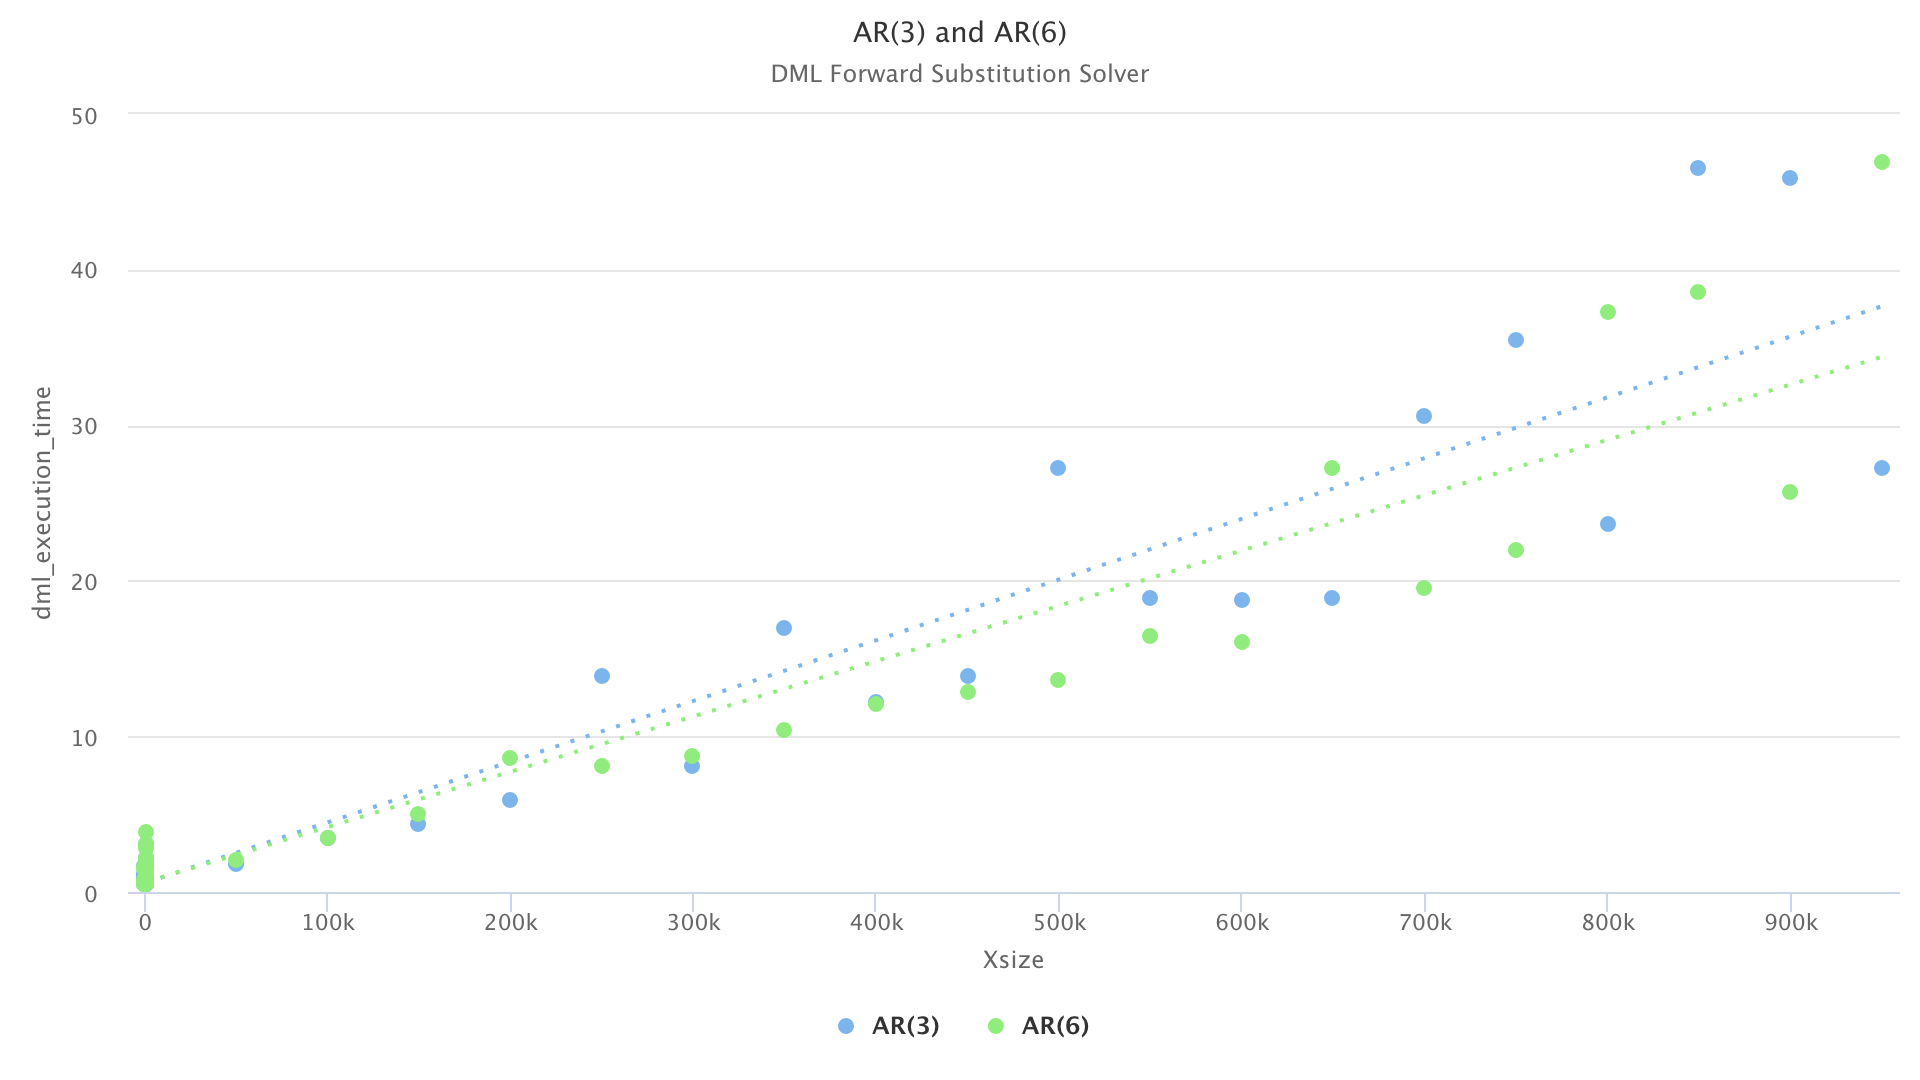
\includegraphics[width=\defaultsizeGraph]{images/ar-comparison-forwardsub.png}}
	\caption{Comparison of \textbf{Execution time} of \textbf{AR(3) and AR(6) for Forward Substitution DML} for time series with sizes \textbf{from $1,000$ up to $950,000$} }
    \label{apx-fig:ar-comparison-forwardsun}
\end{figure}

\begin{figure}[ht]
	\centering
	\scalebox{1}{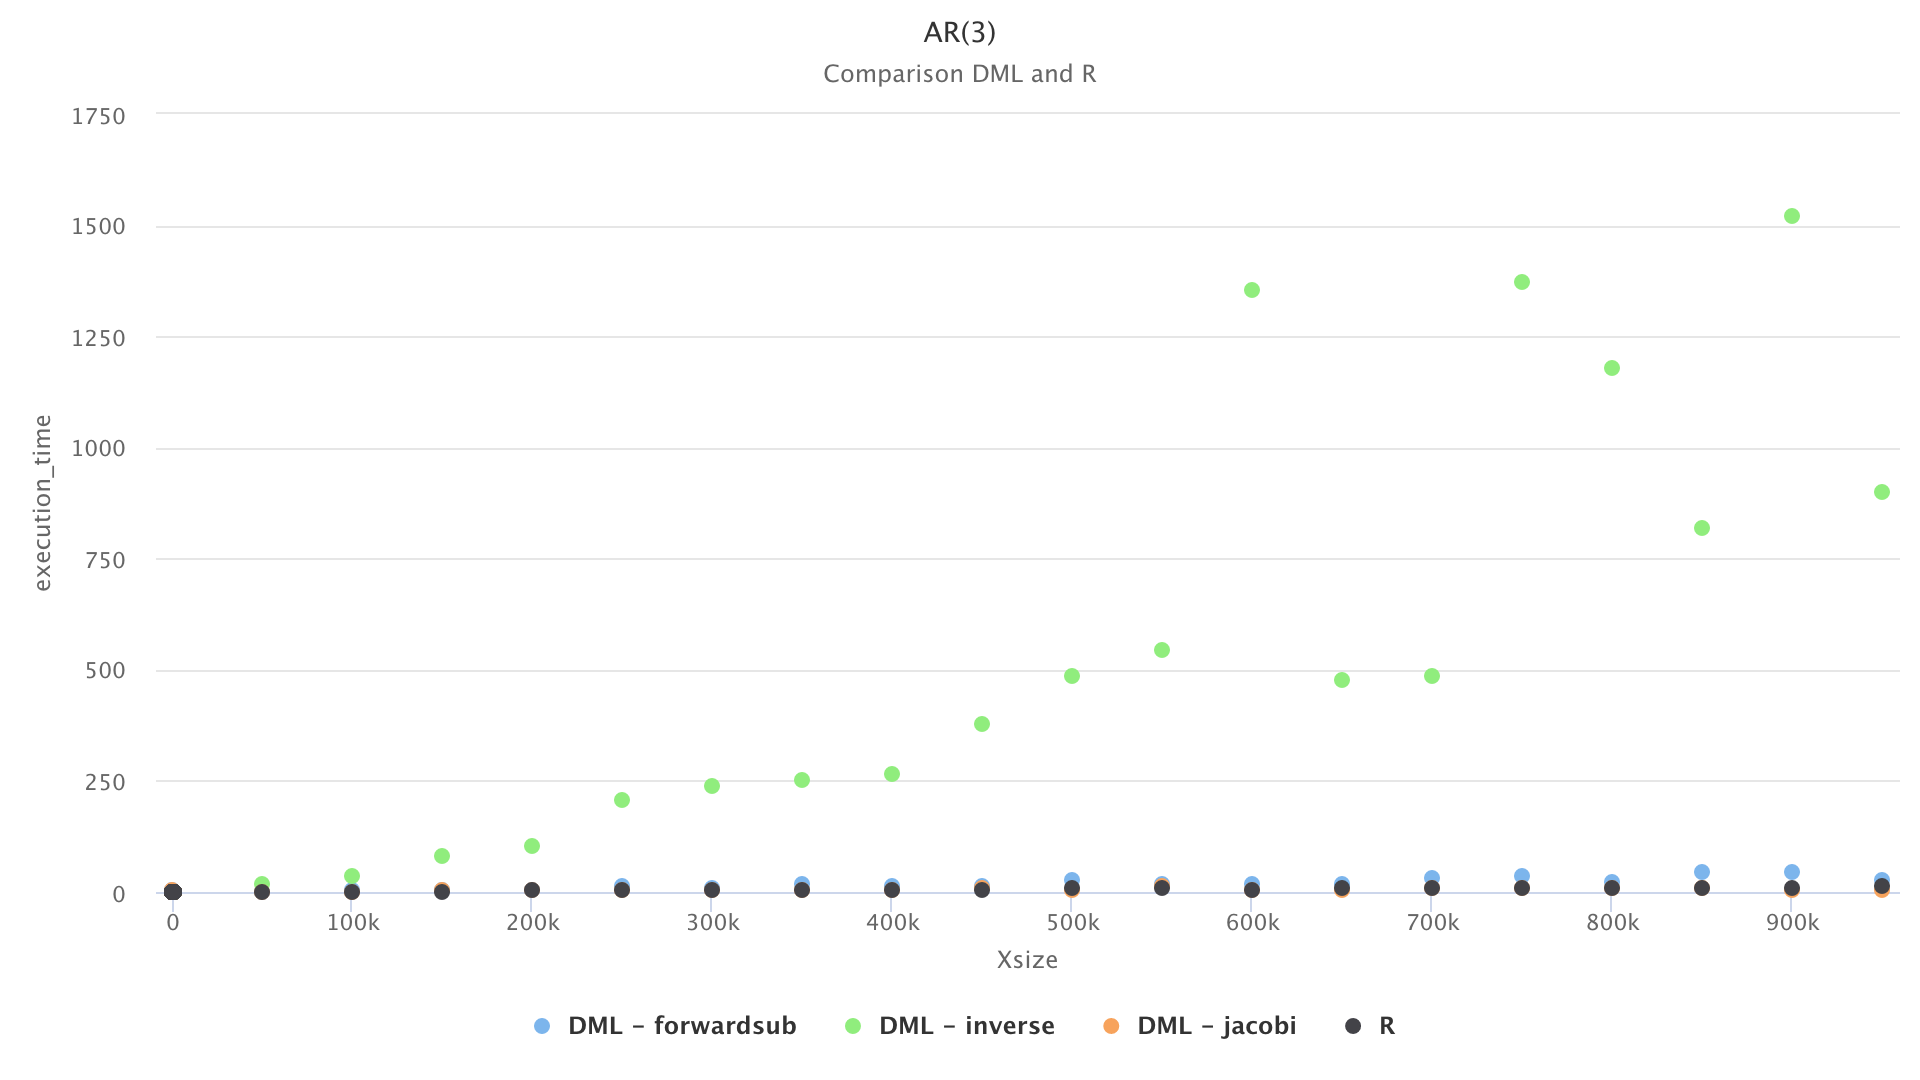
\includegraphics[width=\defaultsizeGraph]{images/ar3-exectime-scatter-all_big.png}}
	\caption{\textbf{Execution time} of AR(3) for DML and R for time series with sizes \textbf{up to $950,000$} }
    \label{apx-fig:ar3-exectime-scatter-all_big}
\end{figure}

\begin{figure}[ht]
	\centering
	\scalebox{1}{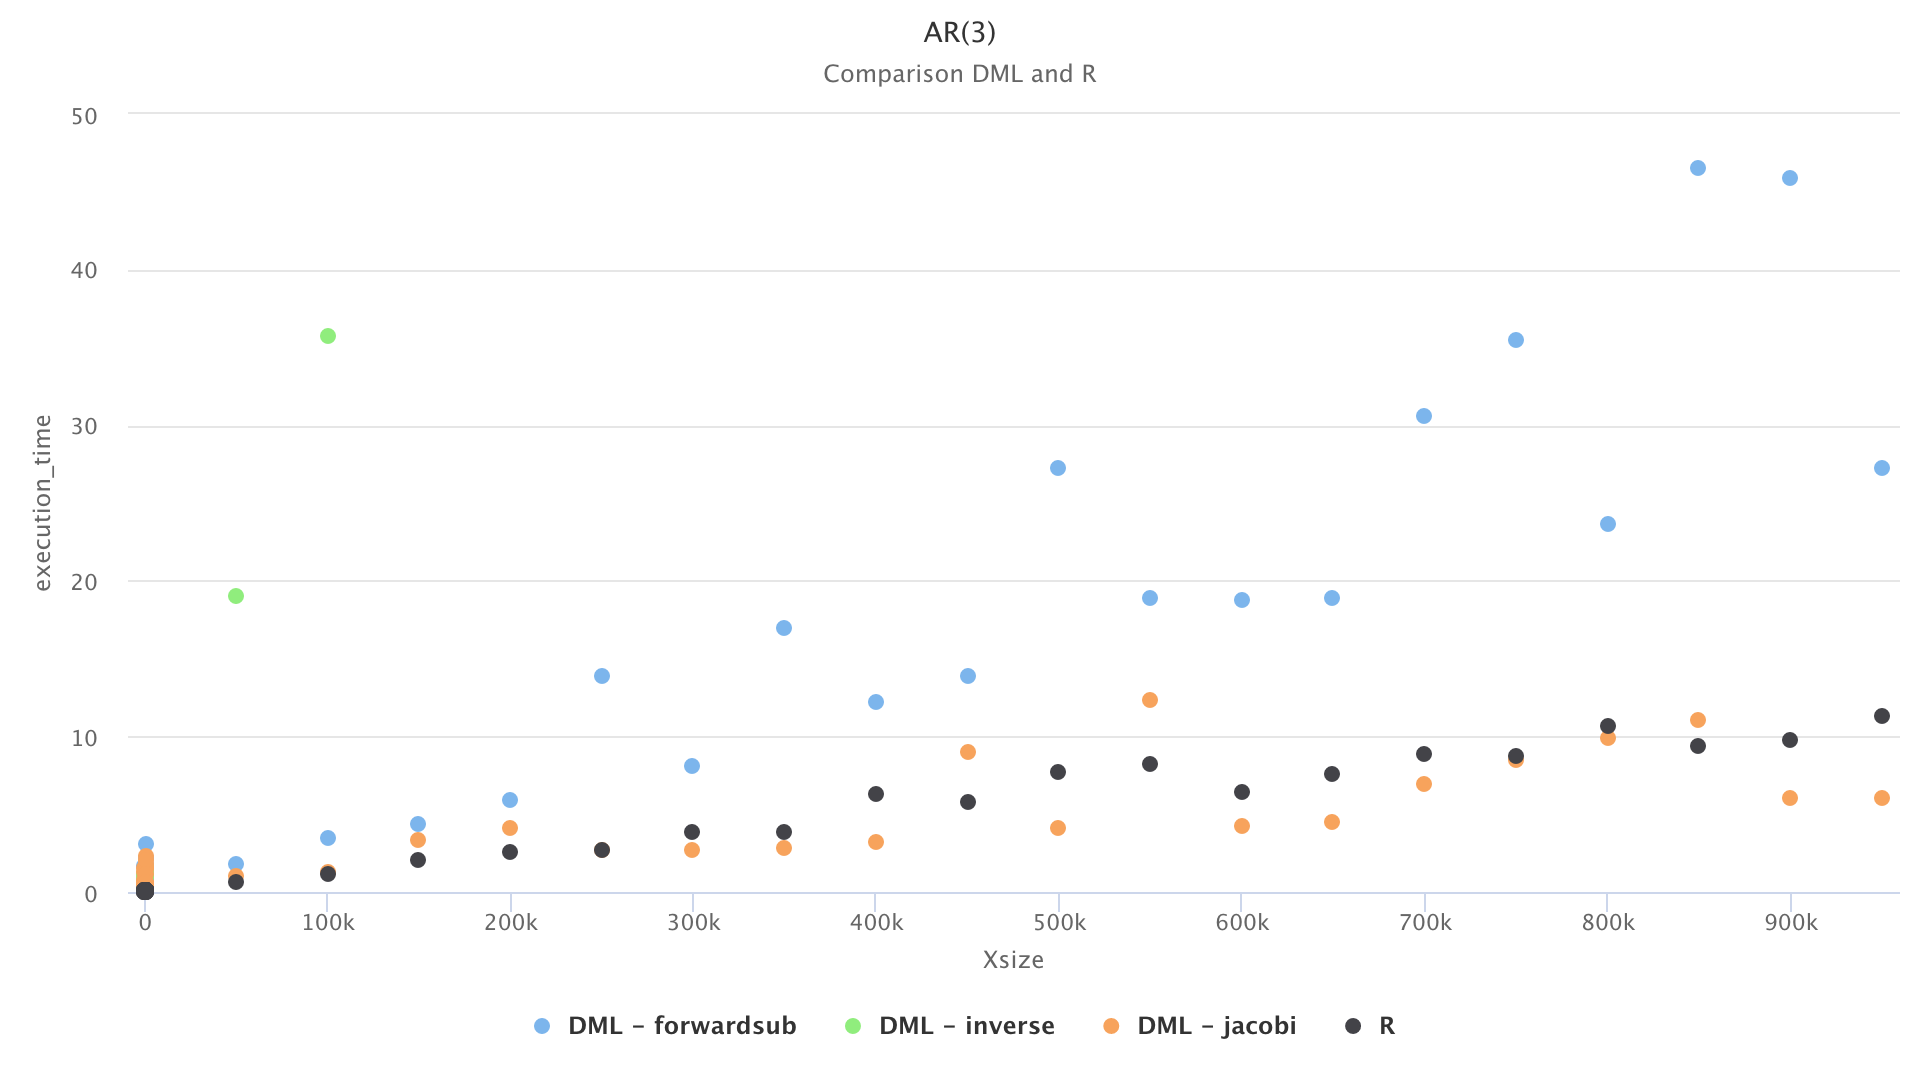
\includegraphics[width=\defaultsizeGraph]{images/ar3-exectime-scatter-all.png}}
	\caption{\textbf{Execution time} of AR(3) for DML and R for time series with sizes \textbf{up to $950,000$} but on a reduced time scale limited to}
    \label{apx-fig:ar3-exectime-scatter-all}
\end{figure}

\begin{figure}[ht]
	\centering
	\scalebox{1}{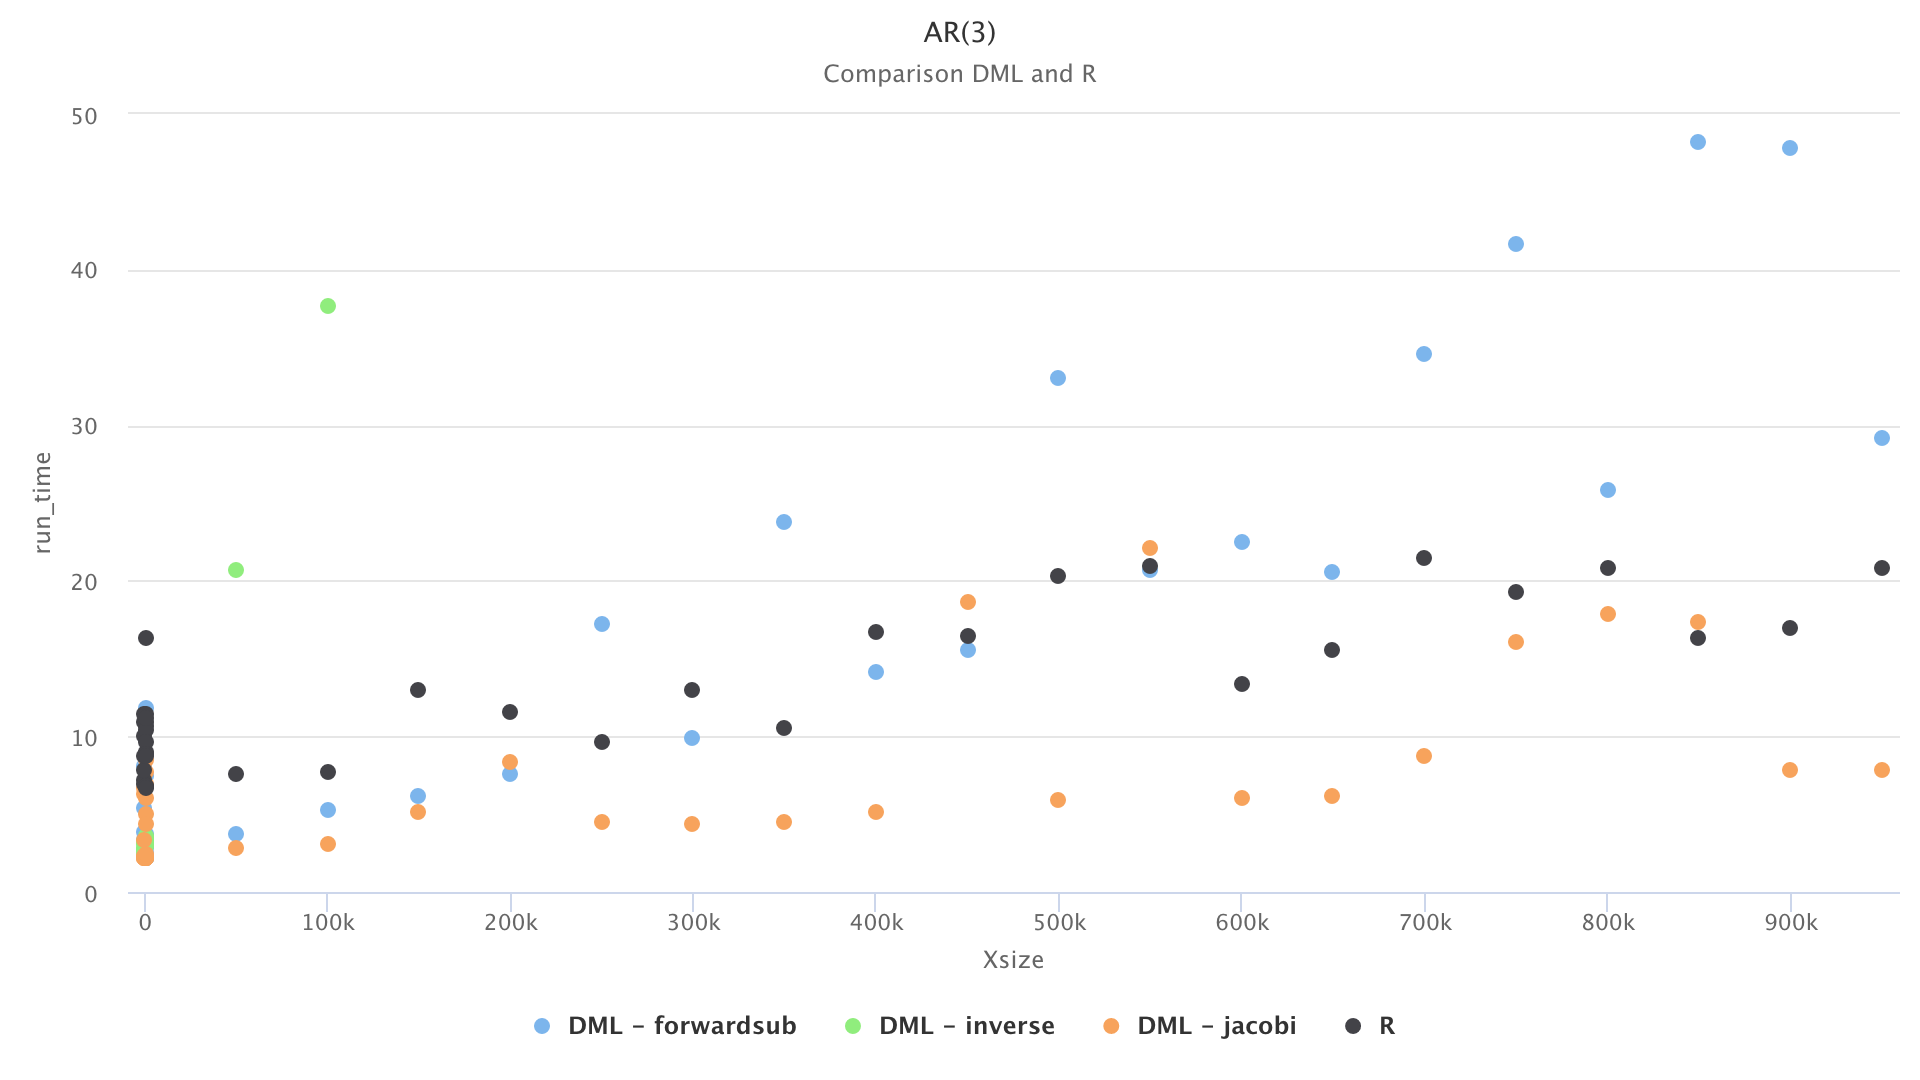
\includegraphics[width=\defaultsizeGraph]{images/ar3-runtime-scatter-all.png}}
	\caption{\textbf{Run time of} AR(3) for DML and R for time series with sizes \textbf{up to $950,000$} }
    \label{apx-fig:ar3-runtime-scatter-all}
\end{figure}

\begin{figure}[ht]
	\centering
	\scalebox{1}{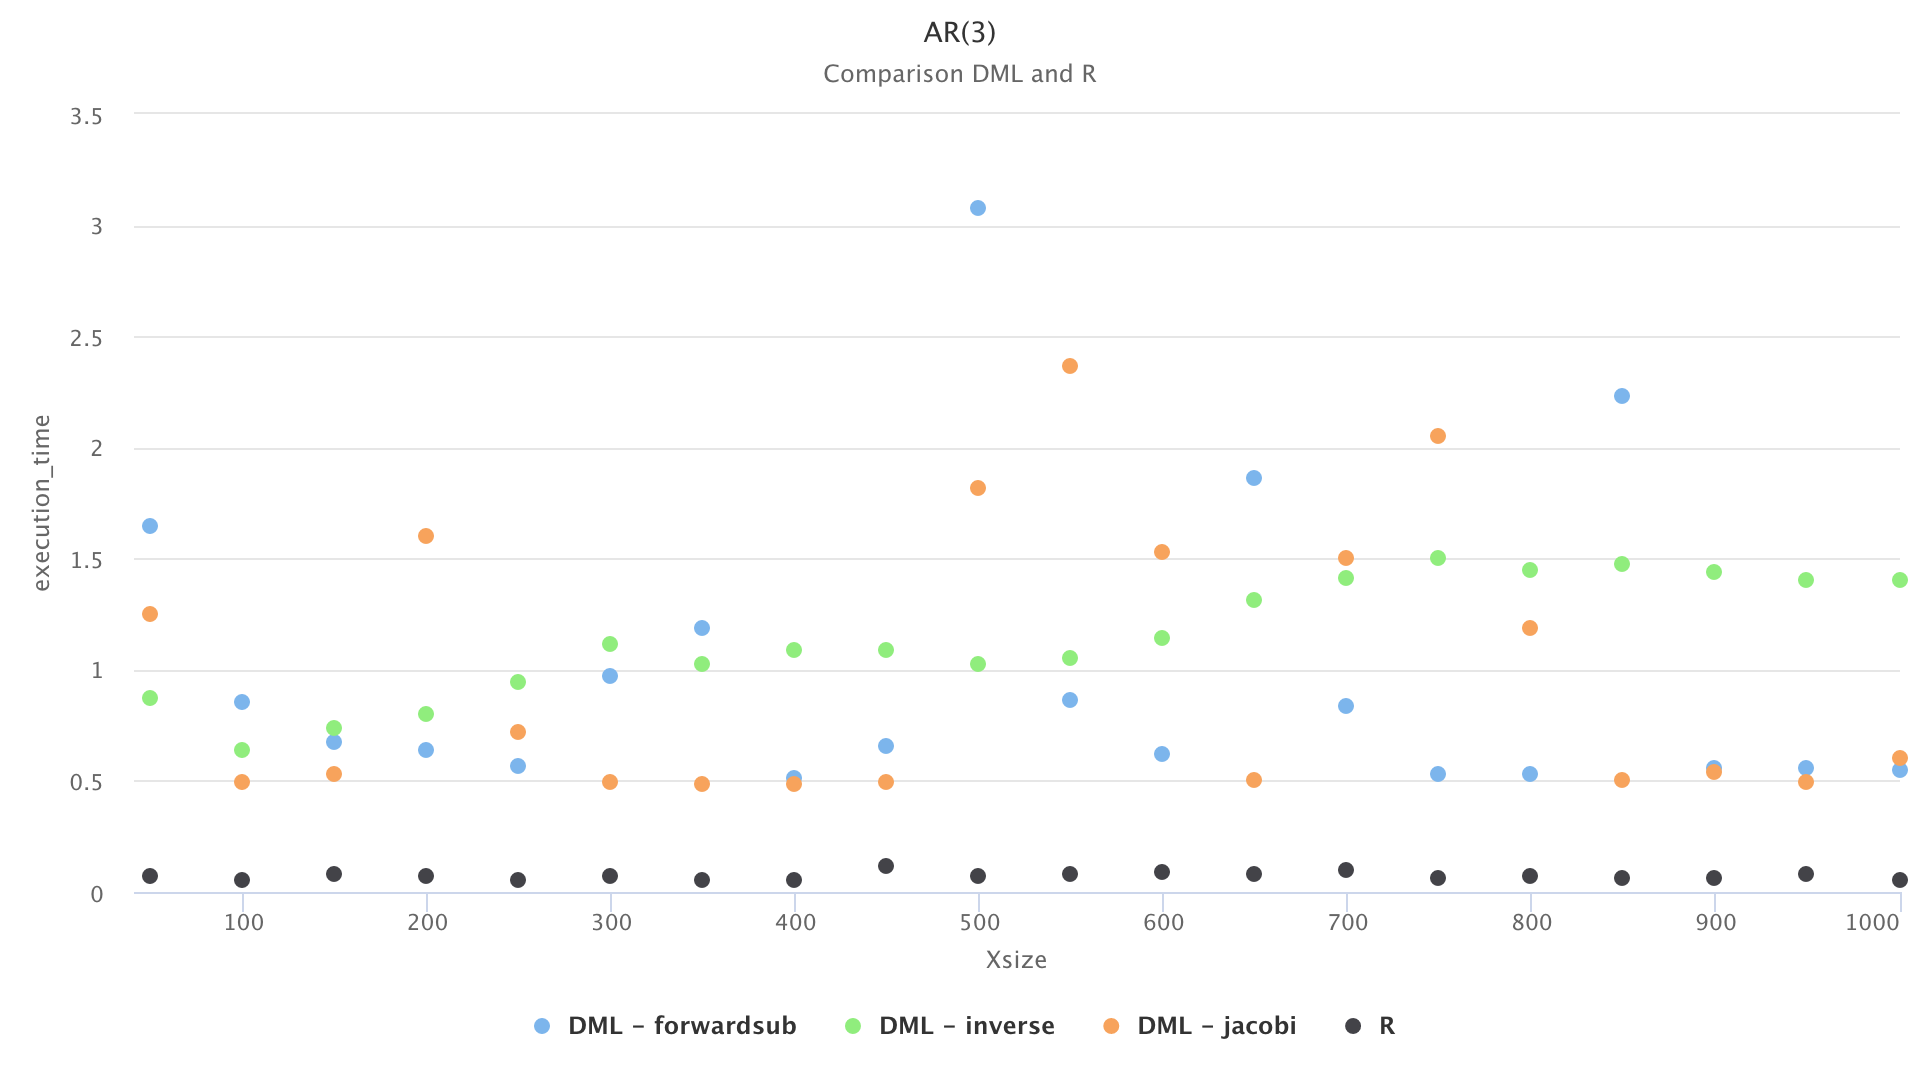
\includegraphics[width=\defaultsizeGraph]{images/ar3-exectime-scatter-all_small.png}}
	\caption{\textbf{Execution time} of AR(3) for DML and R for time series with sizes \textbf{from $50$ to $1,000$} }
    \label{apx-fig:ar3-exectime-scatter-all_small}
\end{figure}

\begin{figure}[ht]
	\centering
	\scalebox{1}{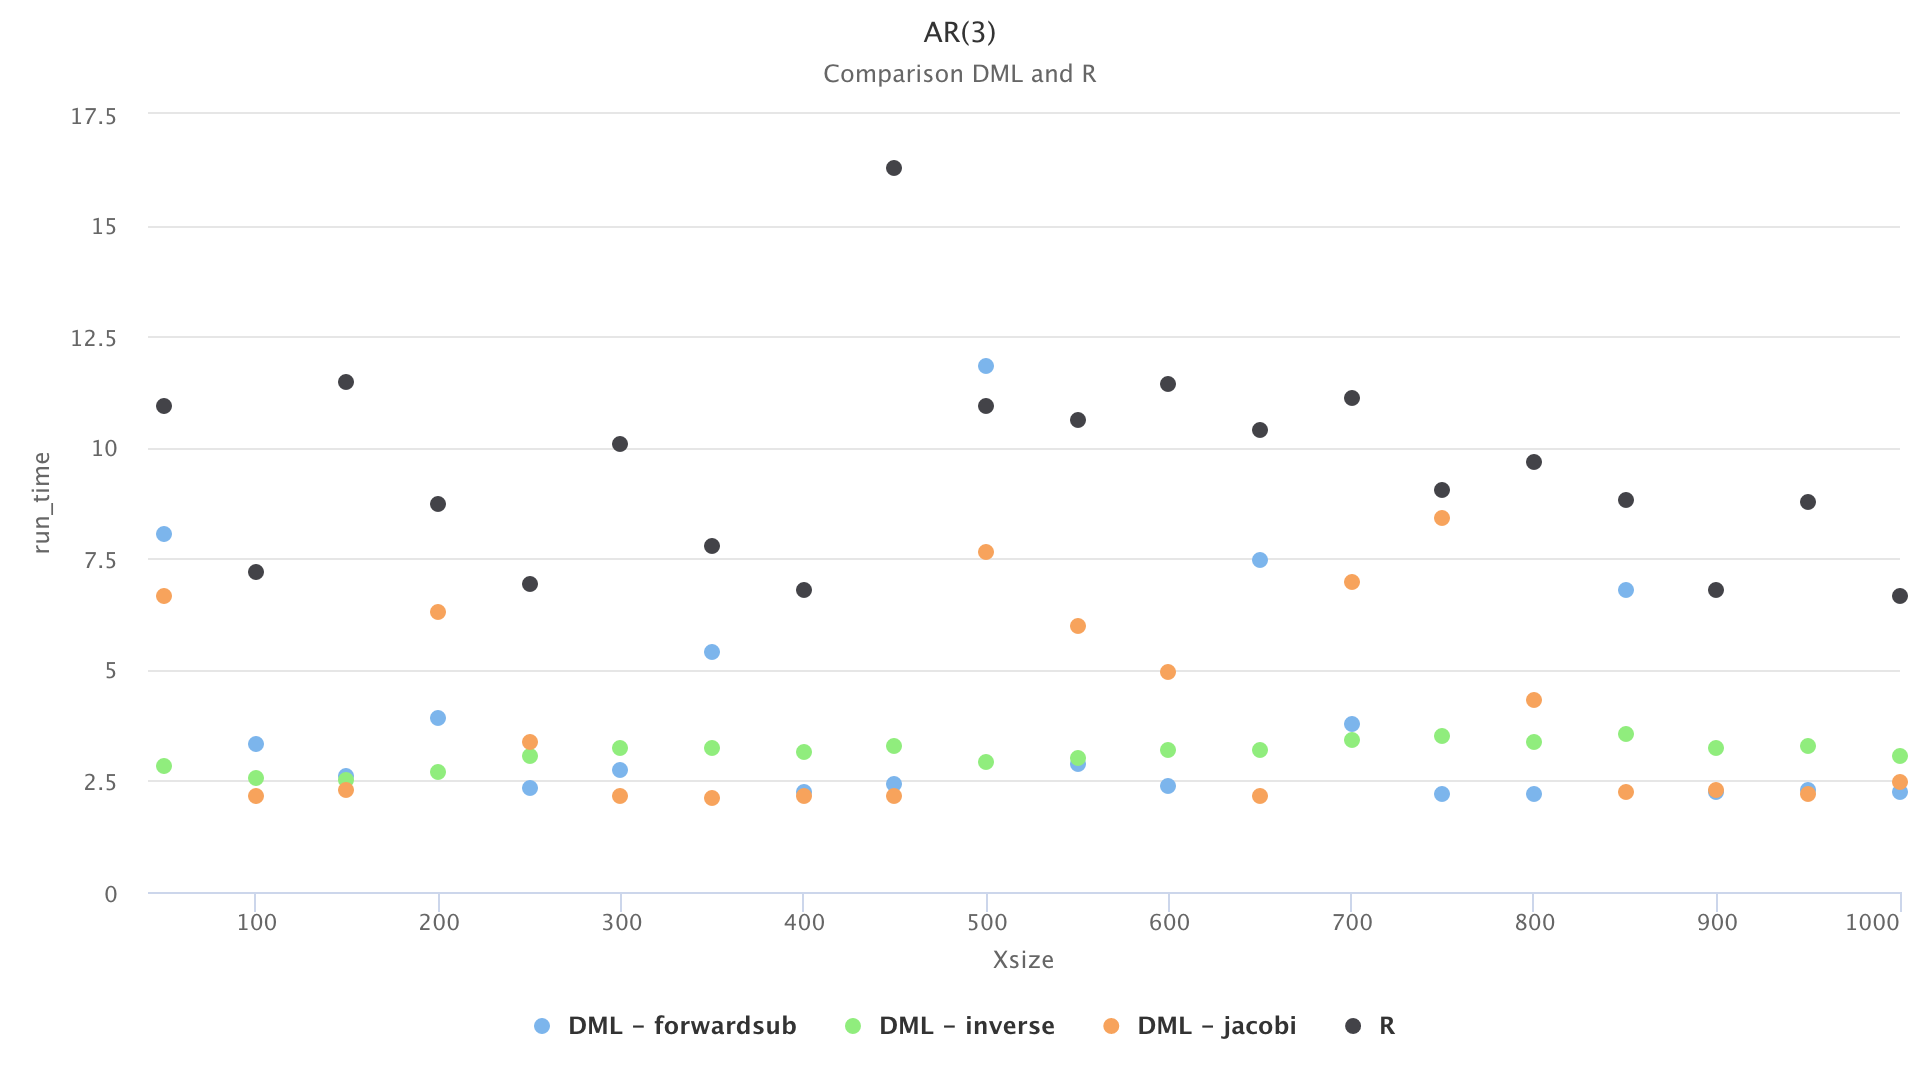
\includegraphics[width=\defaultsizeGraph]{images/ar3-runtime-scatter-all_small.png}}
	\caption{\textbf{Run time} of AR(3) for DML and R for time series with sizes \textbf{from $50$ to $1,000$} }
    \label{apx-fig:ar3-runtime-scatter-all_small}
\end{figure}


\begin{figure}[ht]
	\centering
	\scalebox{1}{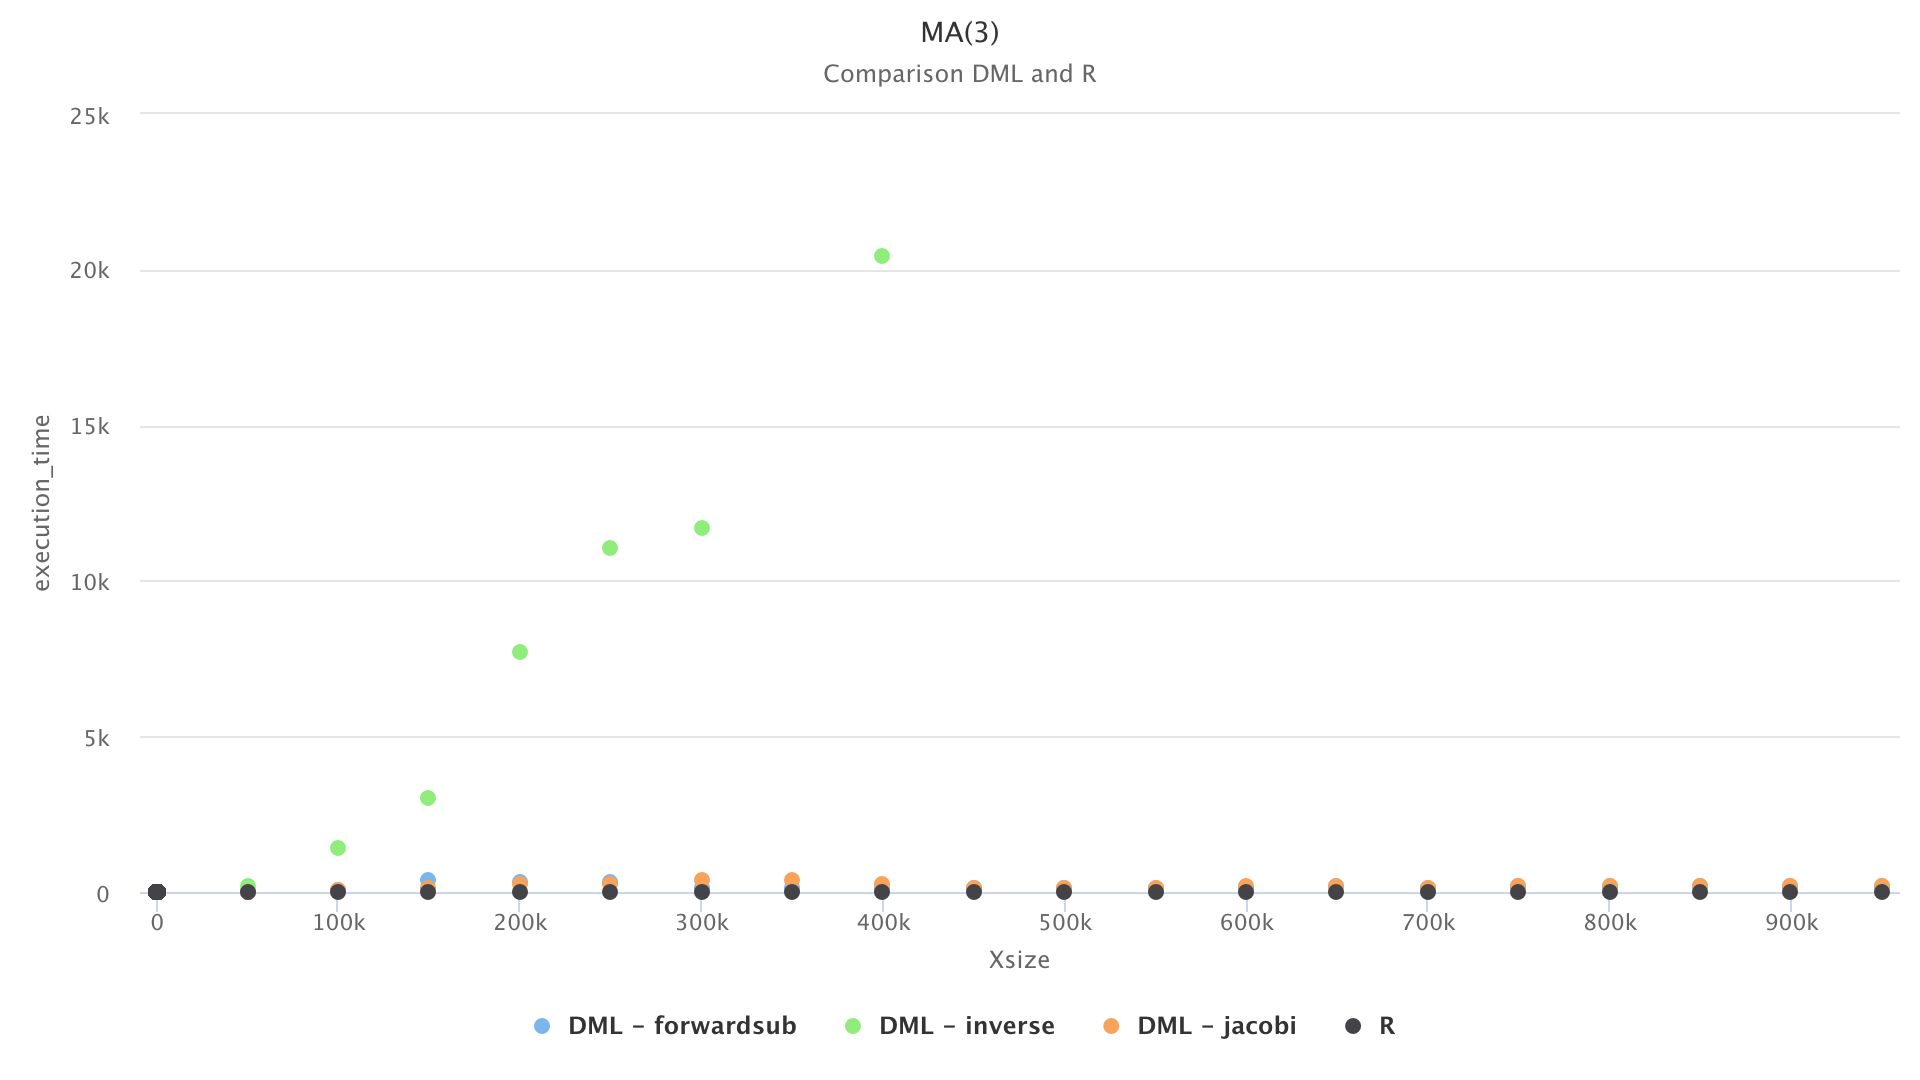
\includegraphics[width=\defaultsizeGraph]{images/ma3-exectime-scatter-all.png}}
	\caption{\textbf{Execution time} of MA(3) for DML and R for time series with sizes \textbf{up to $950,000$} }
    \label{apx-fig:ma3-exectime-scatter-all}
\end{figure}

\begin{figure}[ht]
	\centering
	\scalebox{1}{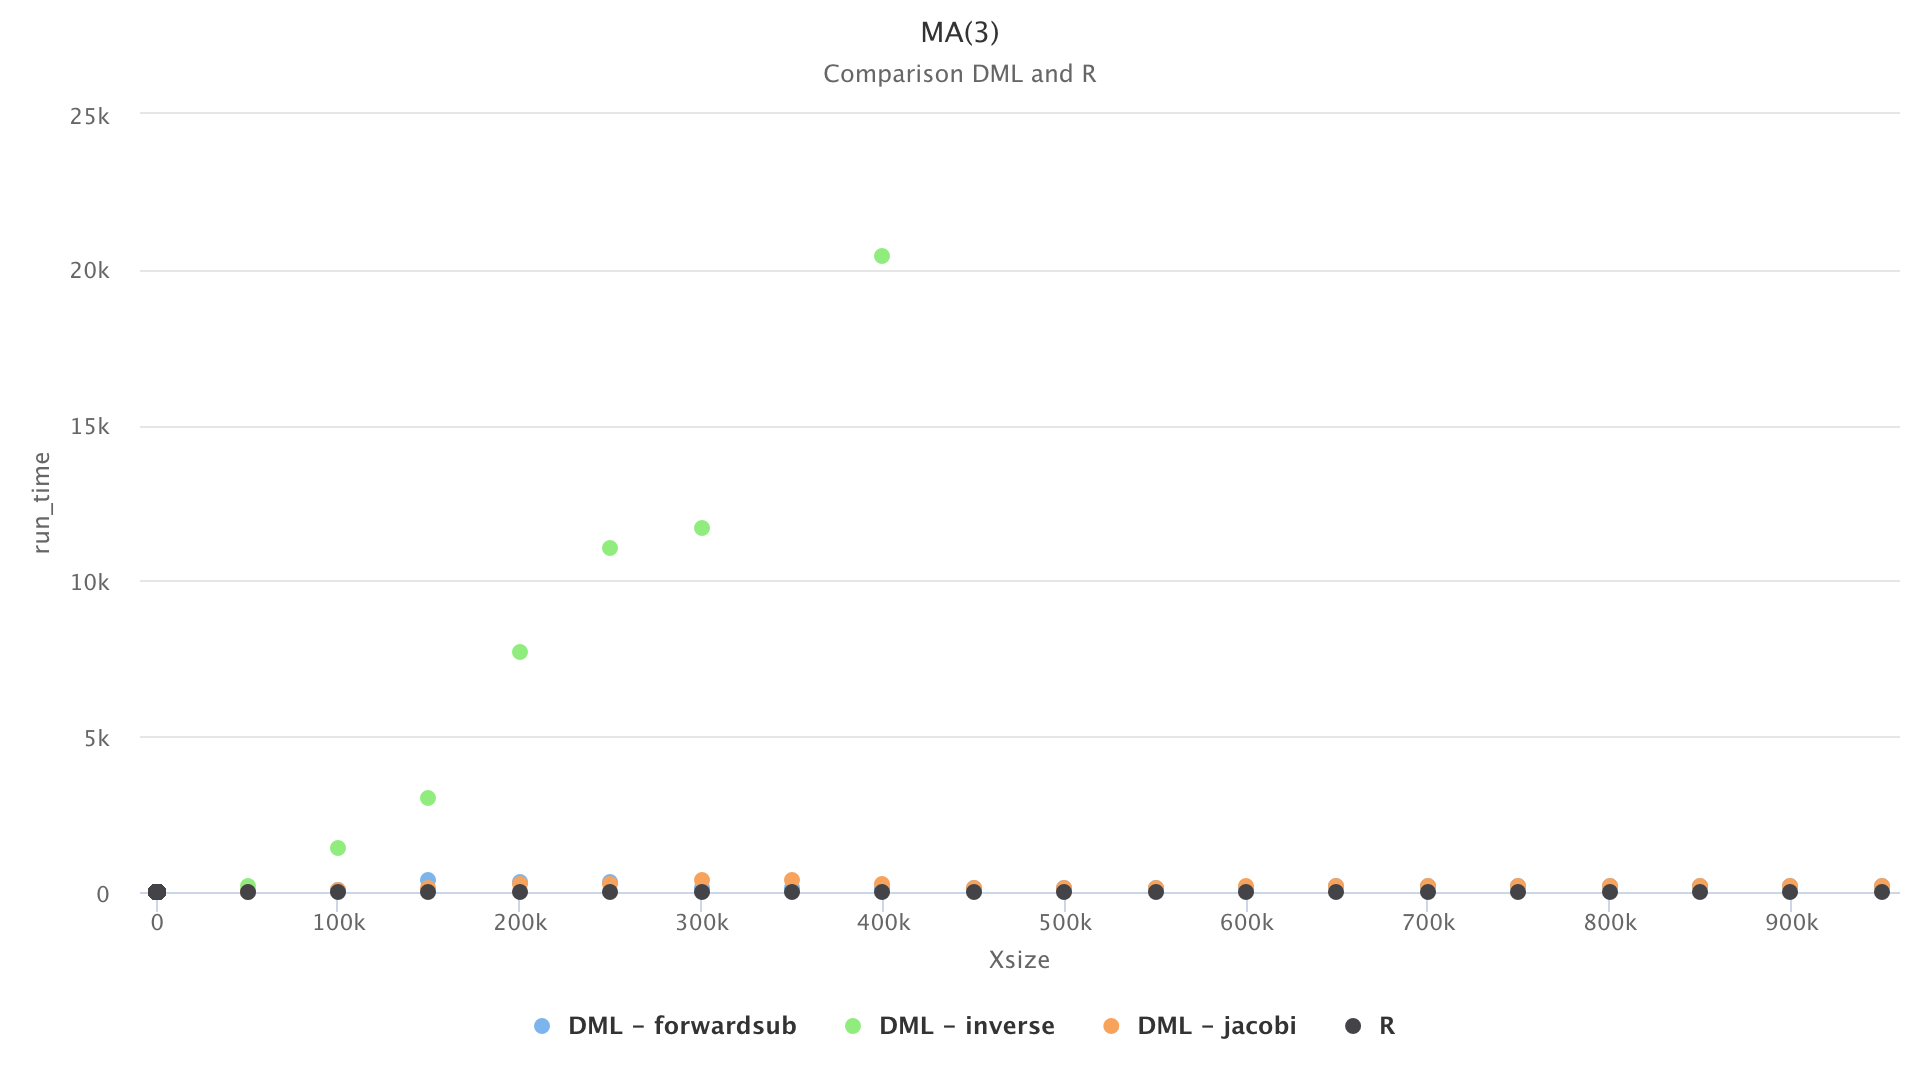
\includegraphics[width=\defaultsizeGraph]{images/ma3-runtime-scatter-all.png}}
	\caption{\textbf{Run time of} MA(3) for DML and R for time series with sizes \textbf{up to $950,000$} }
    \label{apx-fig:ma3-runtime-scatter-all}
\end{figure}

\begin{figure}[ht]
	\centering
	\scalebox{1}{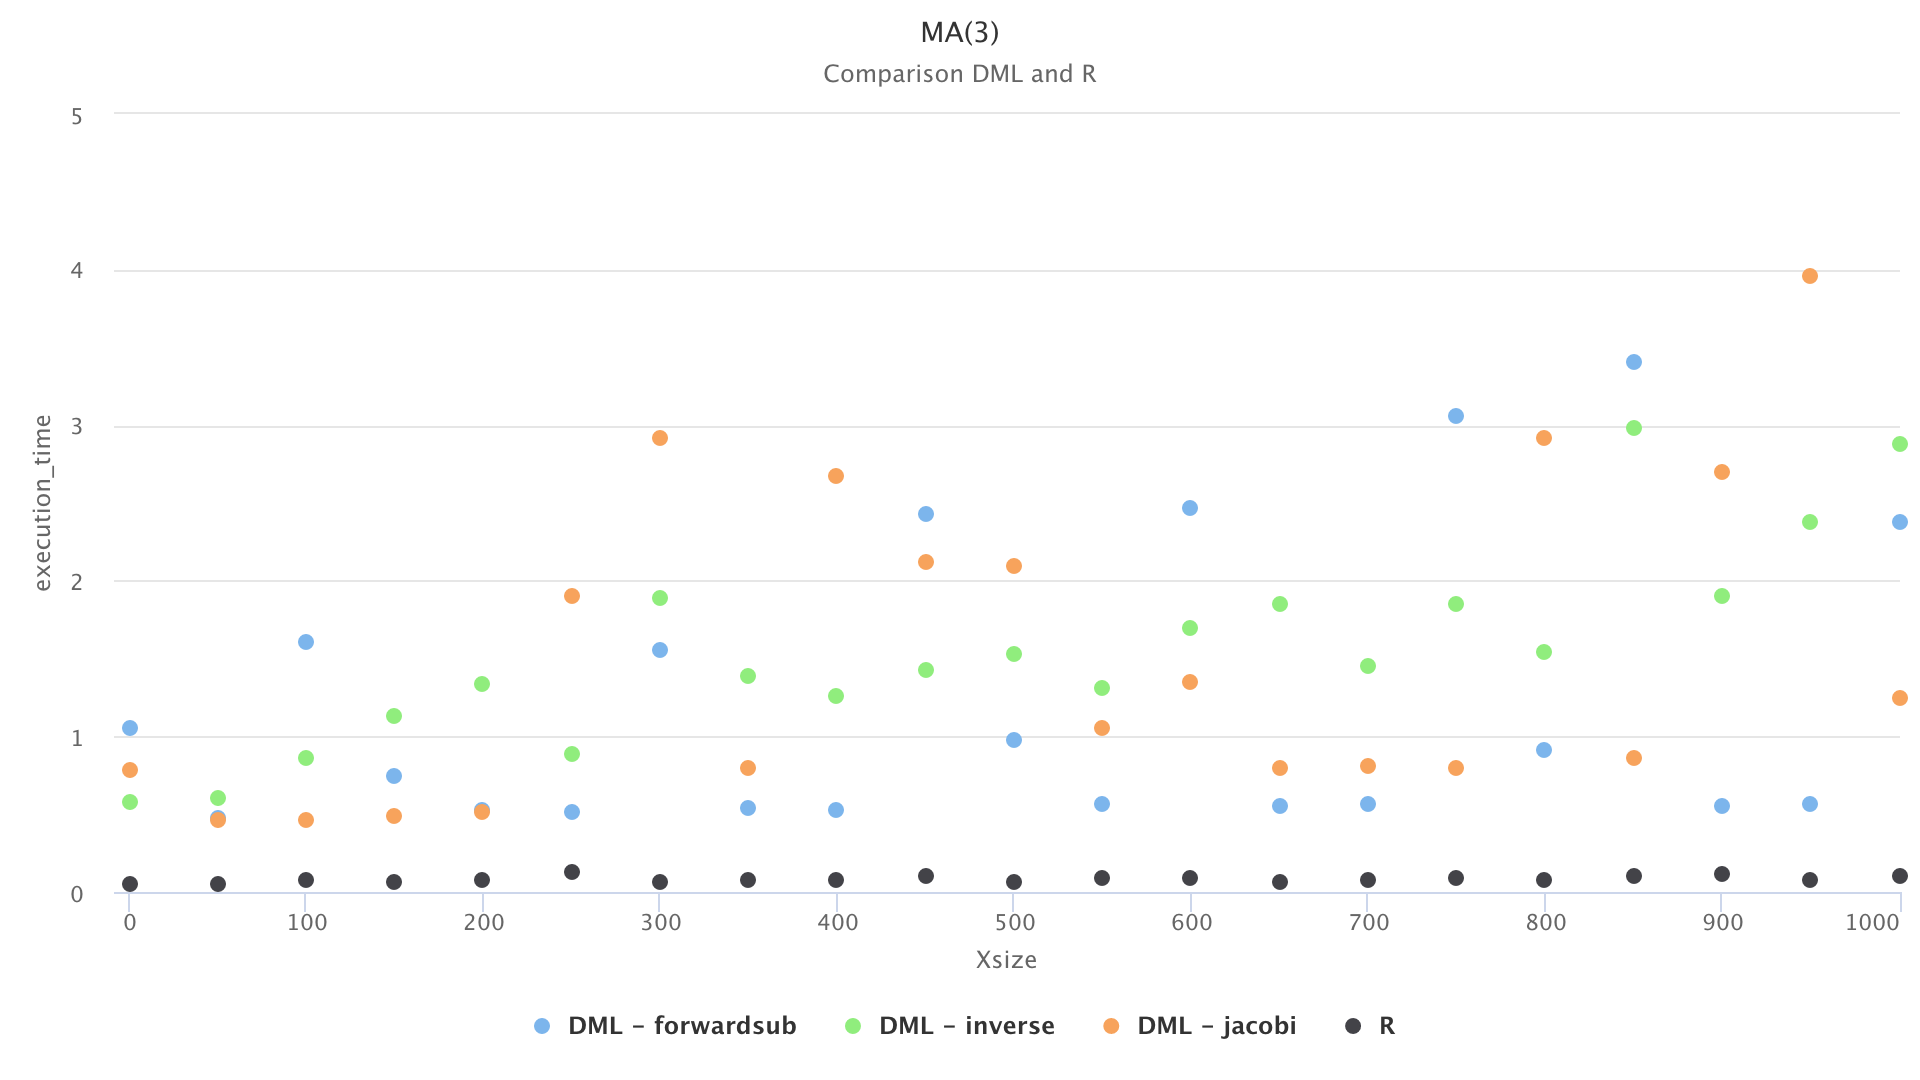
\includegraphics[width=\defaultsizeGraph]{images/ma3-exectime-scatter-all_small.png}}
	\caption{\textbf{Execution time} of MA(3) for DML and R for time series with sizes \textbf{from $50$ to $1,000$} }
    \label{apx-fig:ma3-exectime-scatter-all_small}
\end{figure}

\begin{figure}[ht]
	\centering
	\scalebox{1}{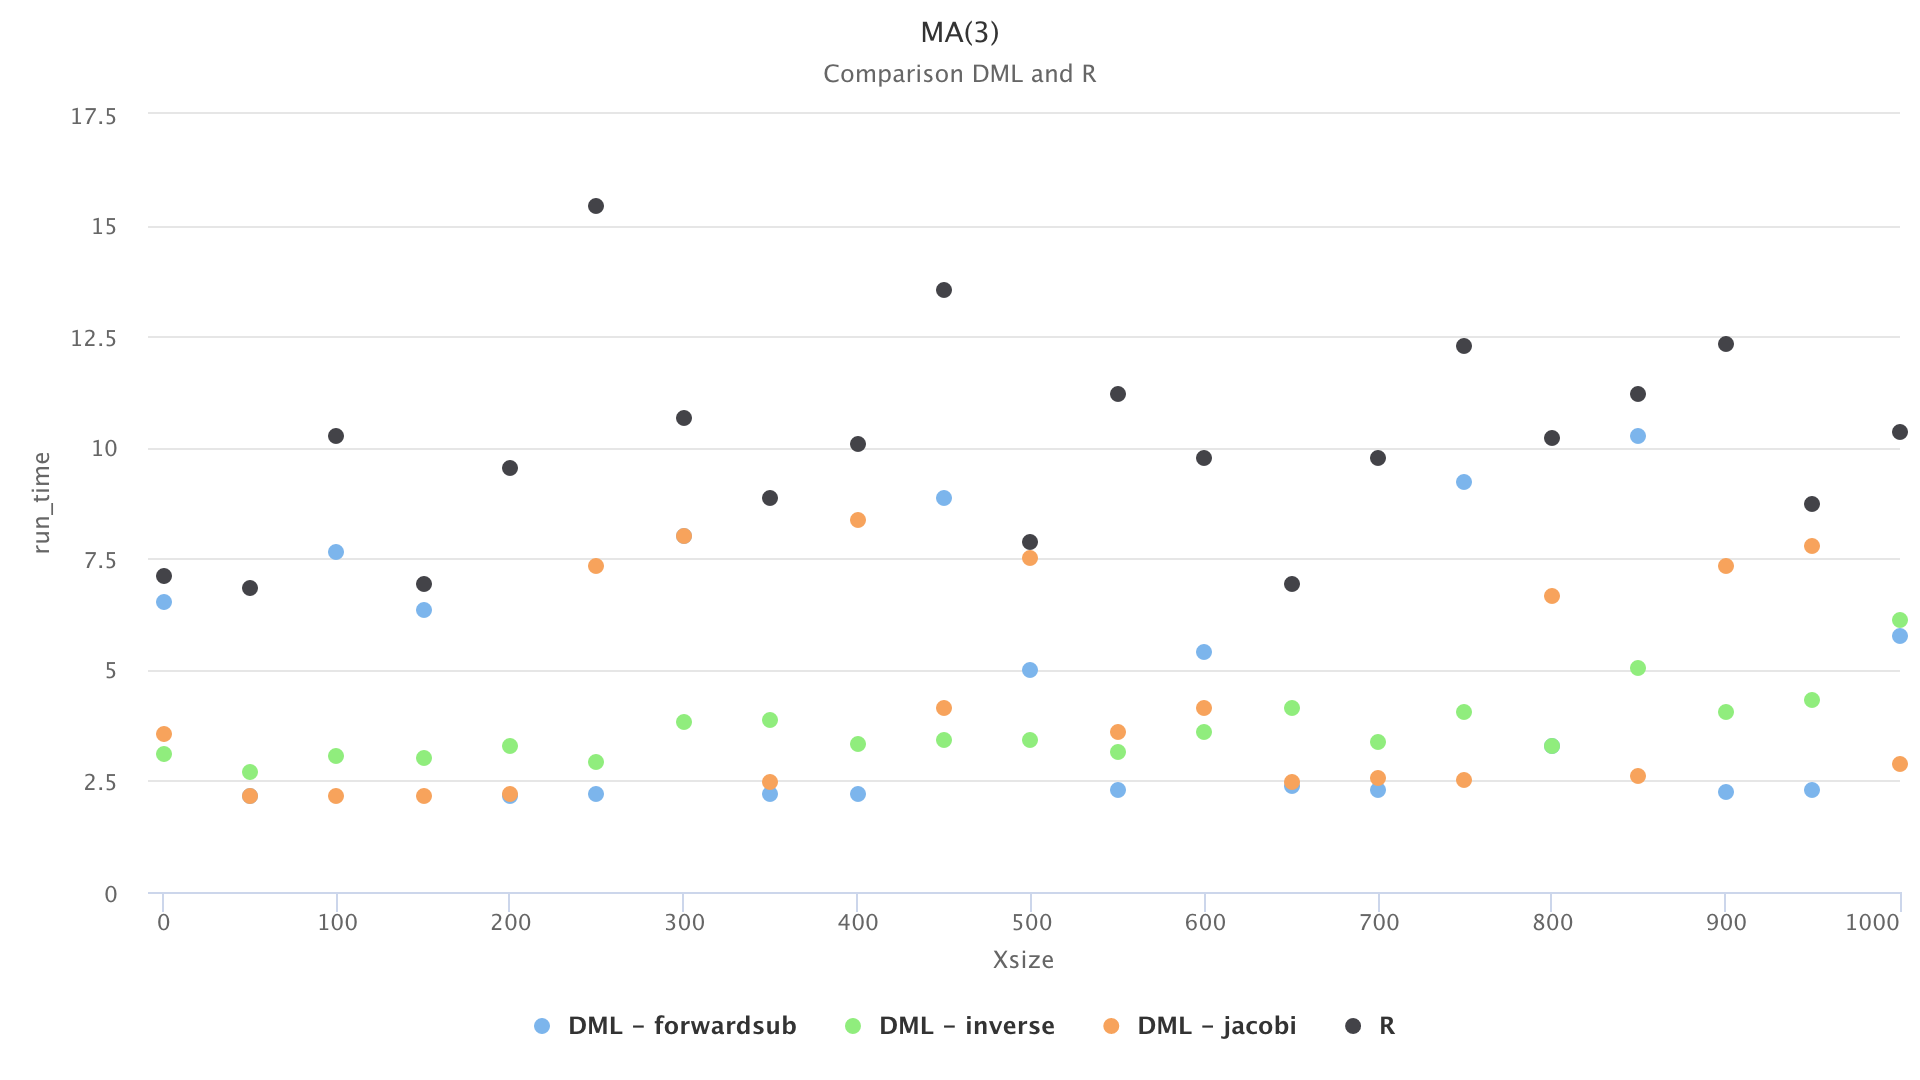
\includegraphics[width=\defaultsizeGraph]{images/ma3-runtime-scatter-all_small.png}}
	\caption{\textbf{Run time} of MA(3) for DML and R for time series with sizes \textbf{from $50$ to $1,000$}}
    \label{apx-fig:ma3-runtime-scatter-all_small}
\end{figure}


\begin{figure}[ht]
	\centering
	\scalebox{1}{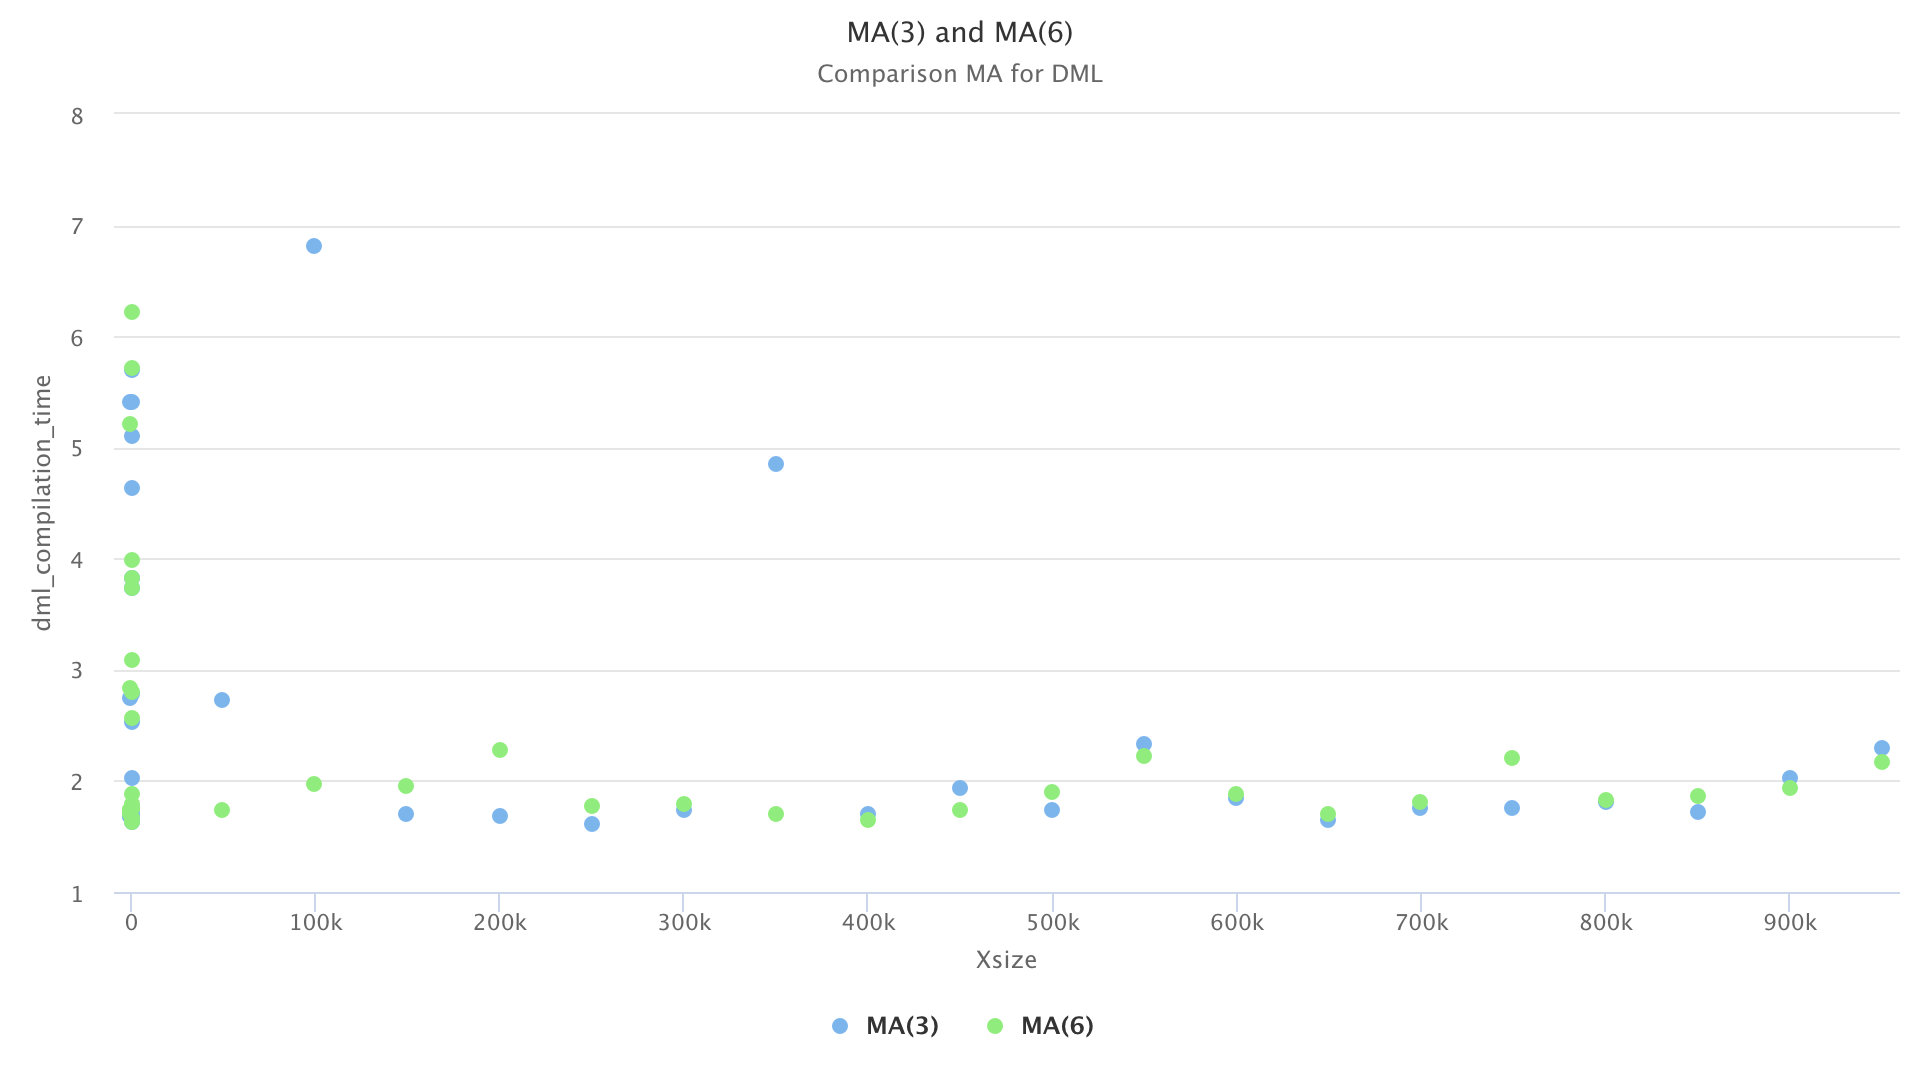
\includegraphics[width=\defaultsizeGraph]{images/ma-comparison.png}}
	\caption{Comparison of DML \textbf{execution time} of MA(3) and MA(6) - \textit{average of all solvers}}
    \label{apx-fig:ma-comparison}
\end{figure}


\begin{figure}[ht]
	\centering
	\scalebox{1}{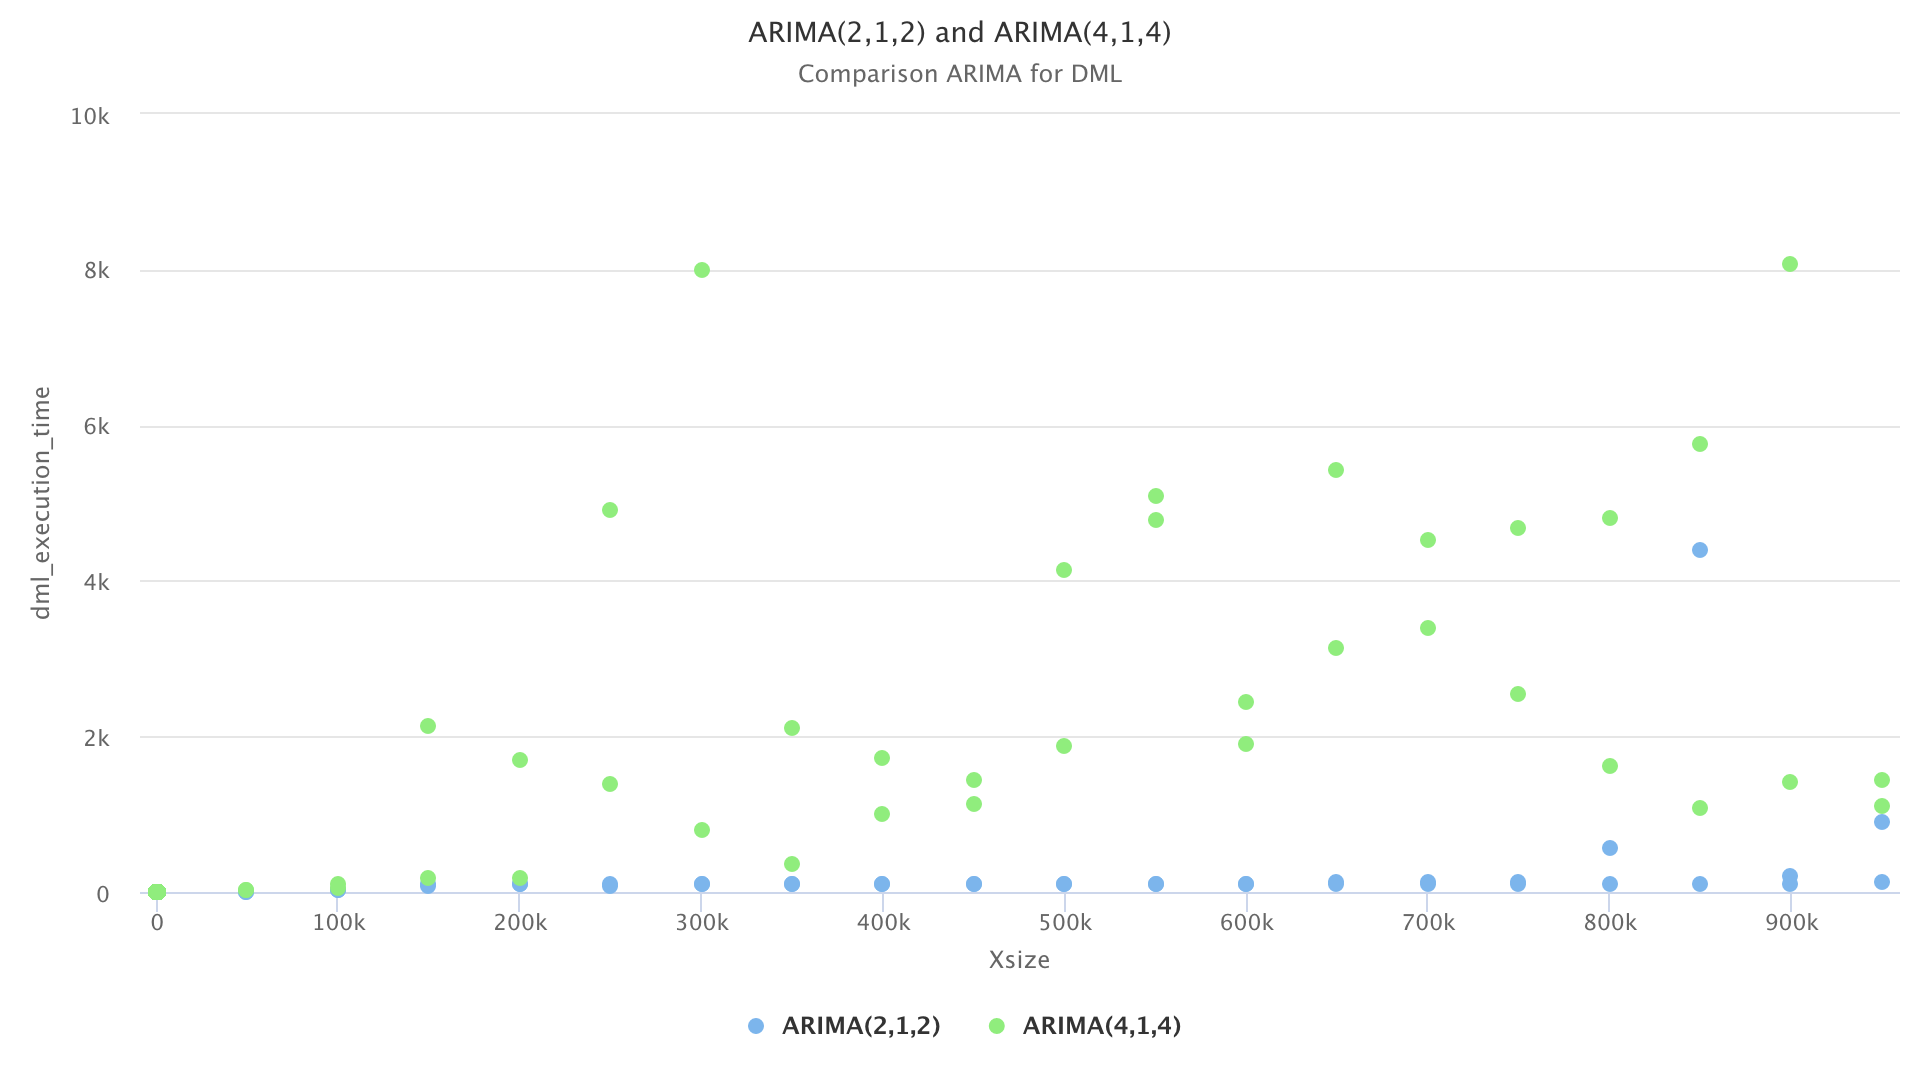
\includegraphics[width=\defaultsizeGraph]{images/arima-comparison.png}}
	\caption{Comparison of DML \textbf{execution time} of ARIMA(2,1,2) and ARIMA(4,1,4) - \textit{average of all solvers}}
    \label{apx-fig:arima-comparison}
\end{figure}


\begin{figure}[ht]
	\centering
	\scalebox{1}{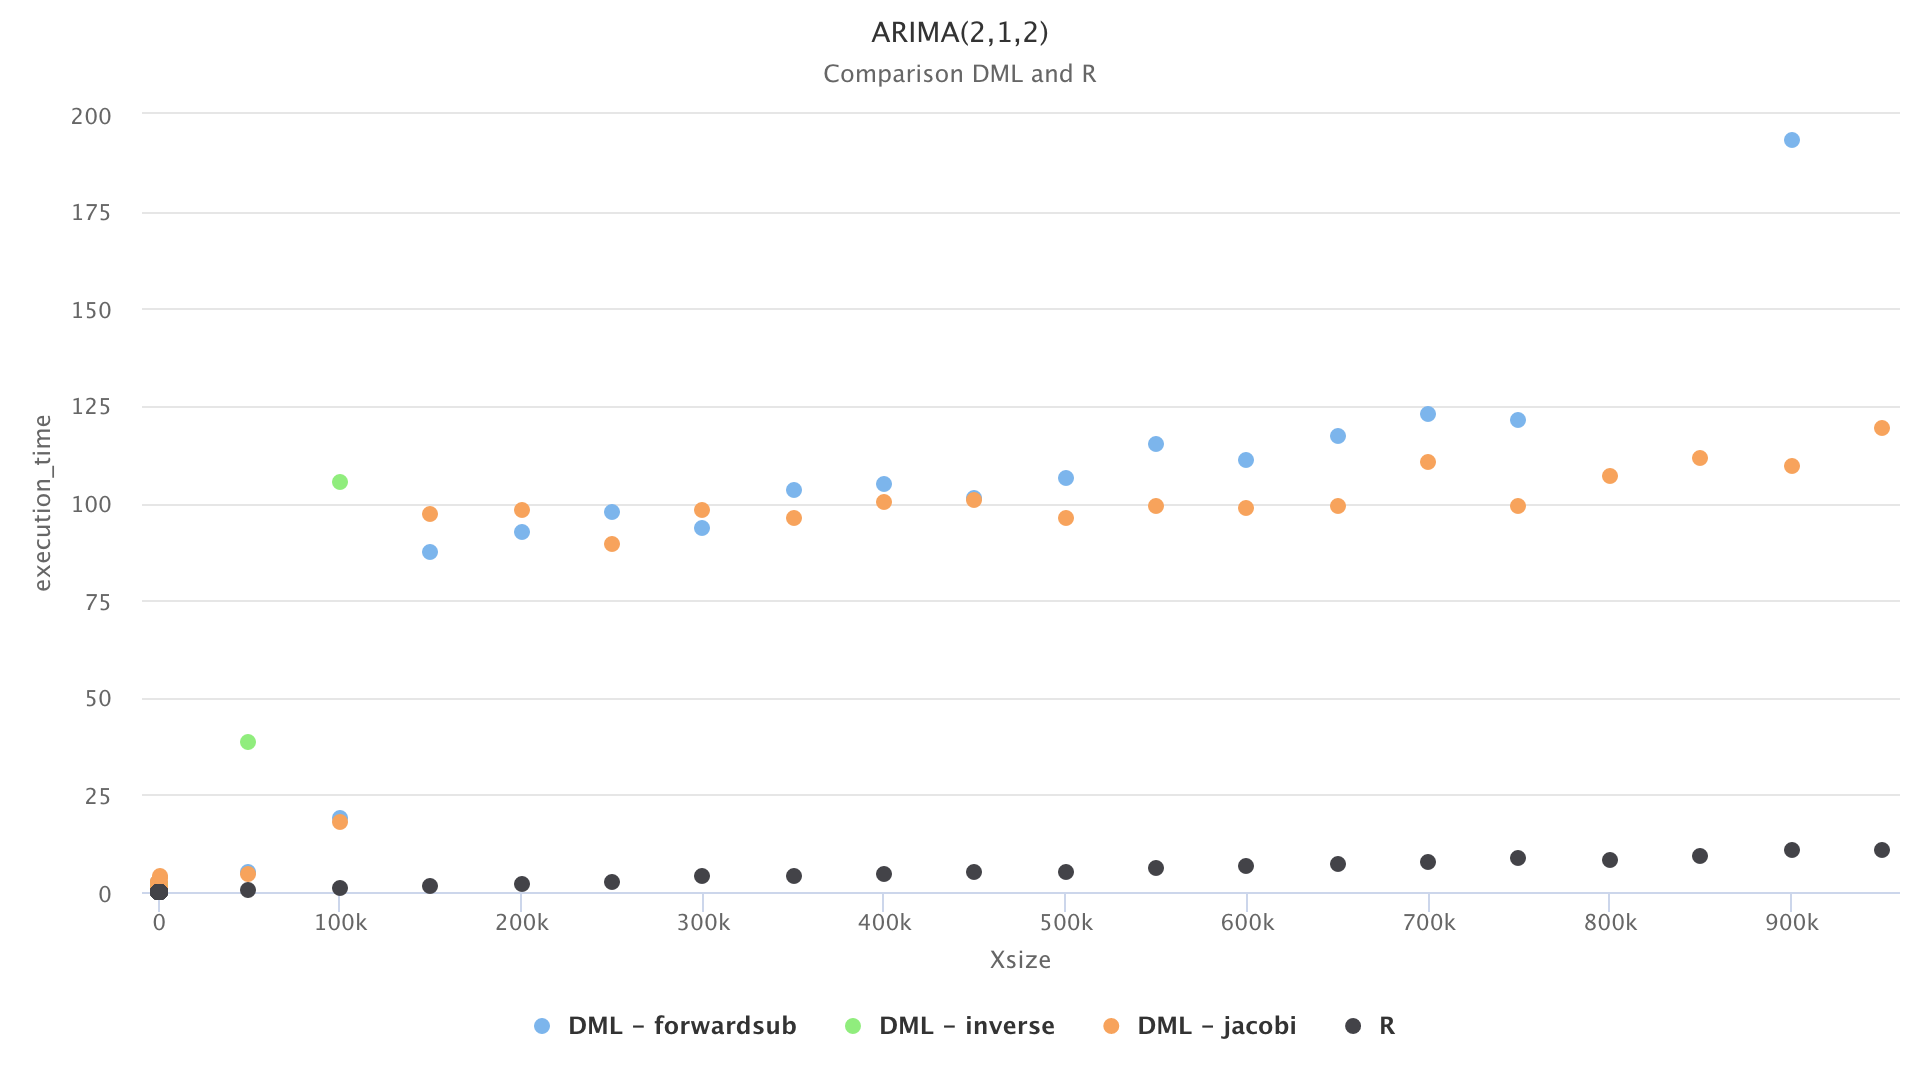
\includegraphics[width=\defaultsizeGraph]{images/arima212-exectime-scatter-all.png}}
	\caption{\textbf{Execution time} of ARIMA(2,1,2) for DML and R for time series with sizes \textbf{up to $950,000$} }
    \label{apx-fig:arima212-exectime-scatter-all}
\end{figure}

\begin{figure}[ht]
	\centering
	\scalebox{1}{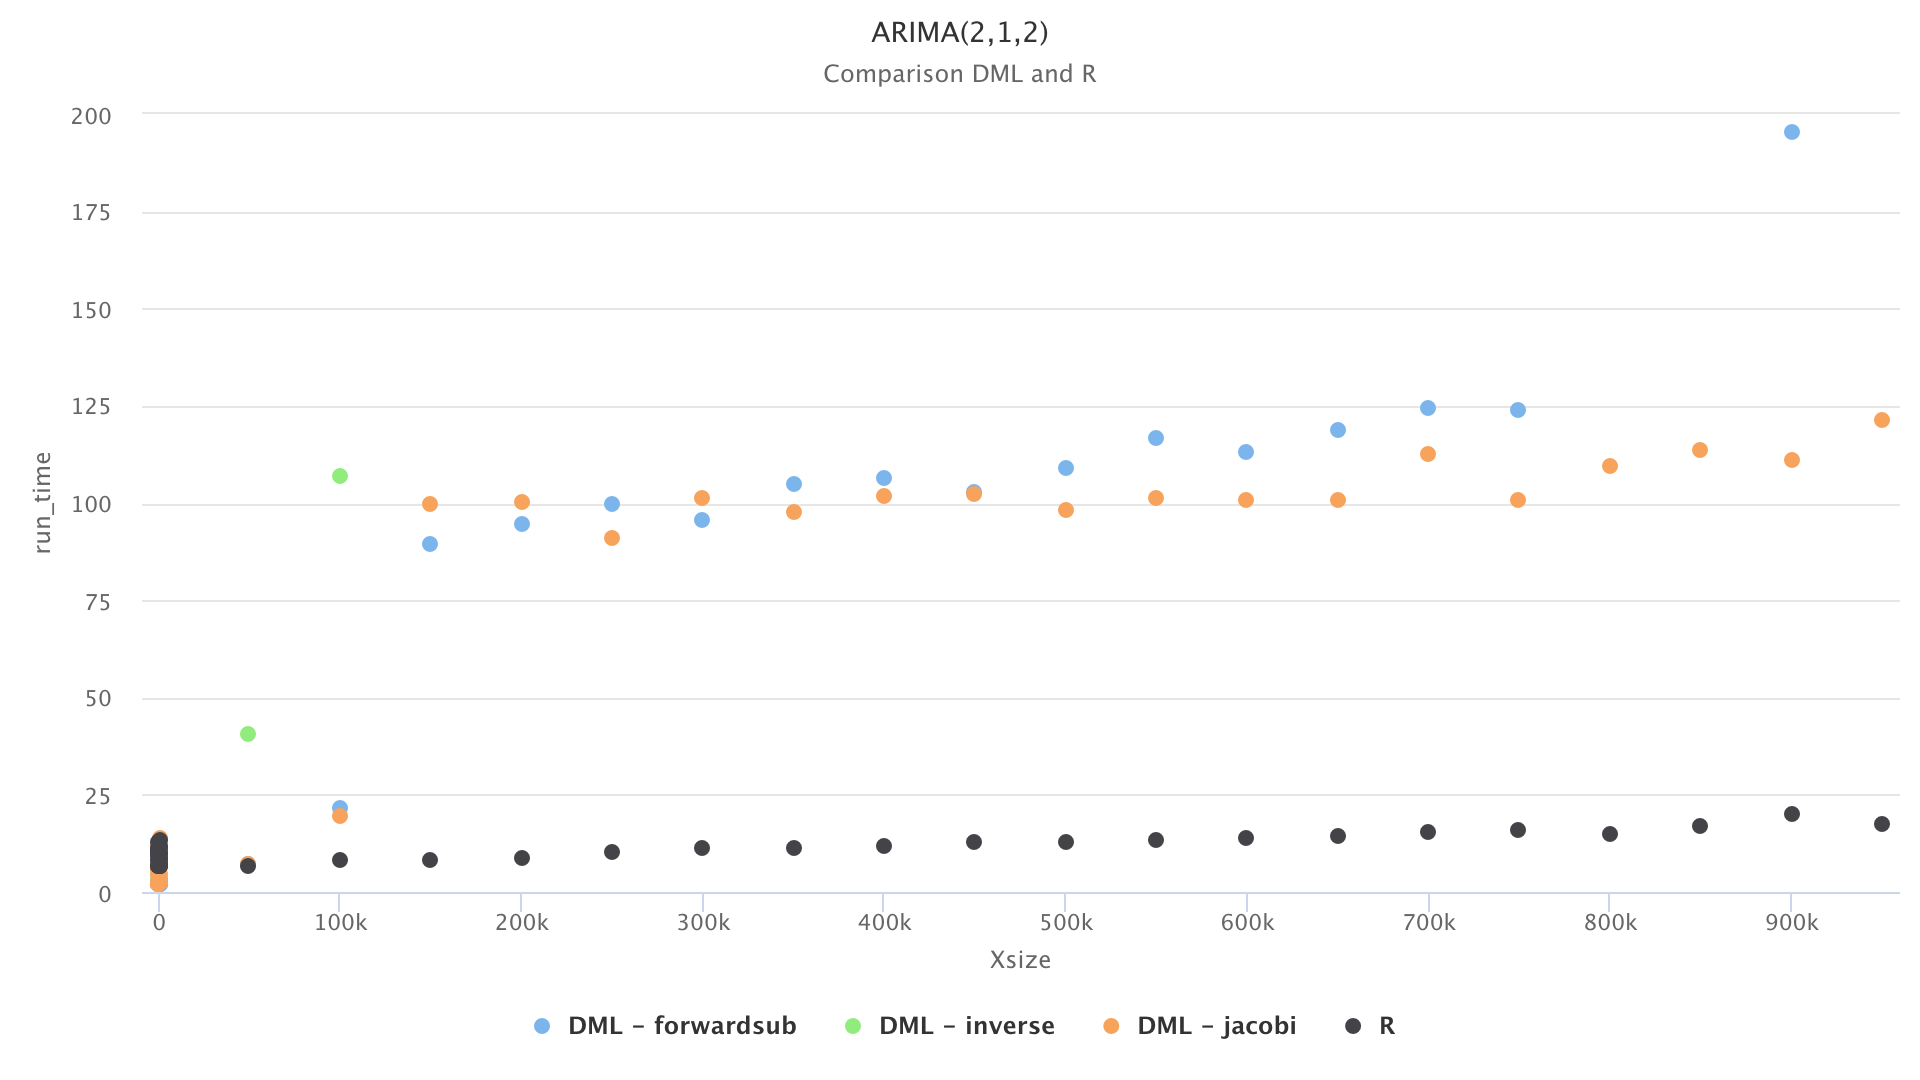
\includegraphics[width=\defaultsizeGraph]{images/arima212-runtime-scatter-all.png}}
	\caption{\textbf{Run time of} ARIMA(2,1,2) for DML and R for time series with sizes \textbf{up to $950,000$} }
    \label{apx-fig:arima212-runtime-scatter-all}
\end{figure}

\begin{figure}[ht]
	\centering
	\scalebox{1}{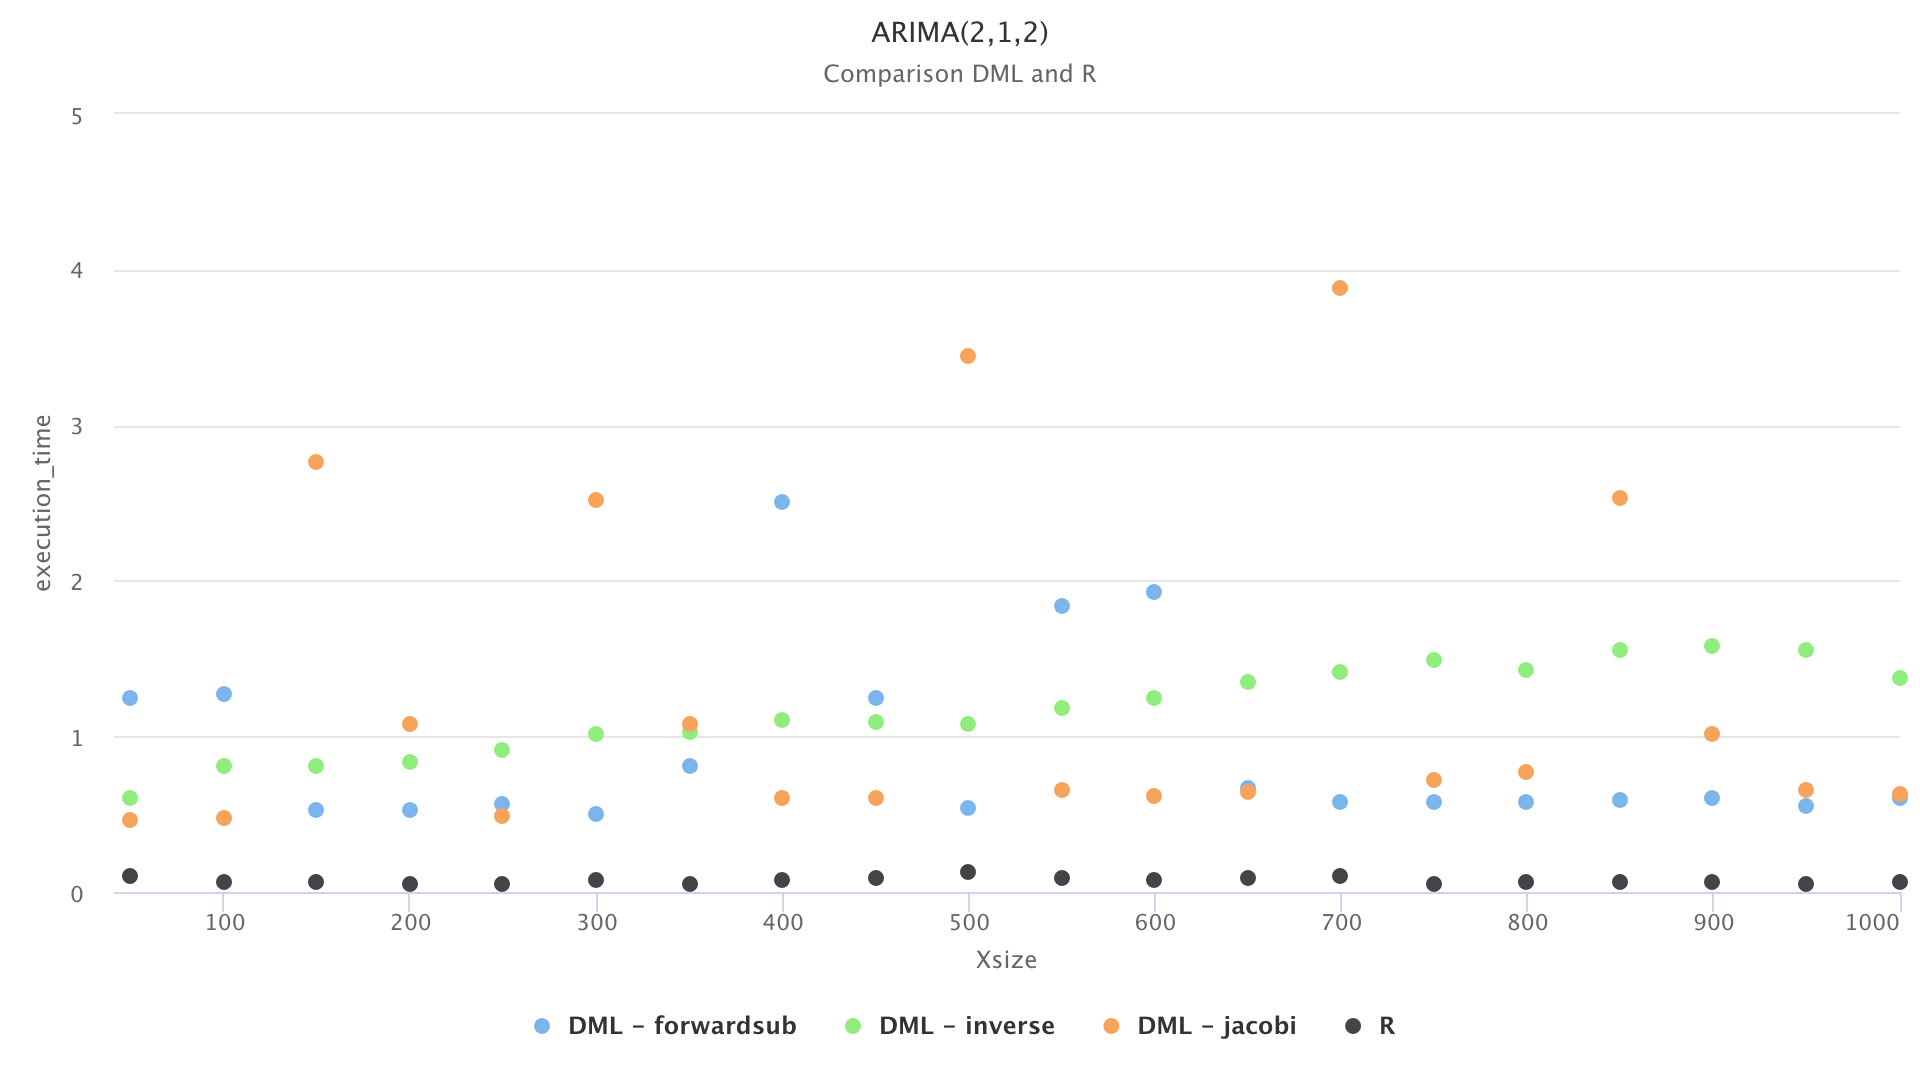
\includegraphics[width=\defaultsizeGraph]{images/arima212-exectime-scatter-all_small.png}}
	\caption{\textbf{Execution time} of ARIMA(2,1,2) for DML and R for time series with sizes \textbf{from $50$ to $1,000$} }
    \label{apx-fig:arima212-exectime-scatter-all_small}
\end{figure}

\begin{figure}[ht]
	\centering
	\scalebox{1}{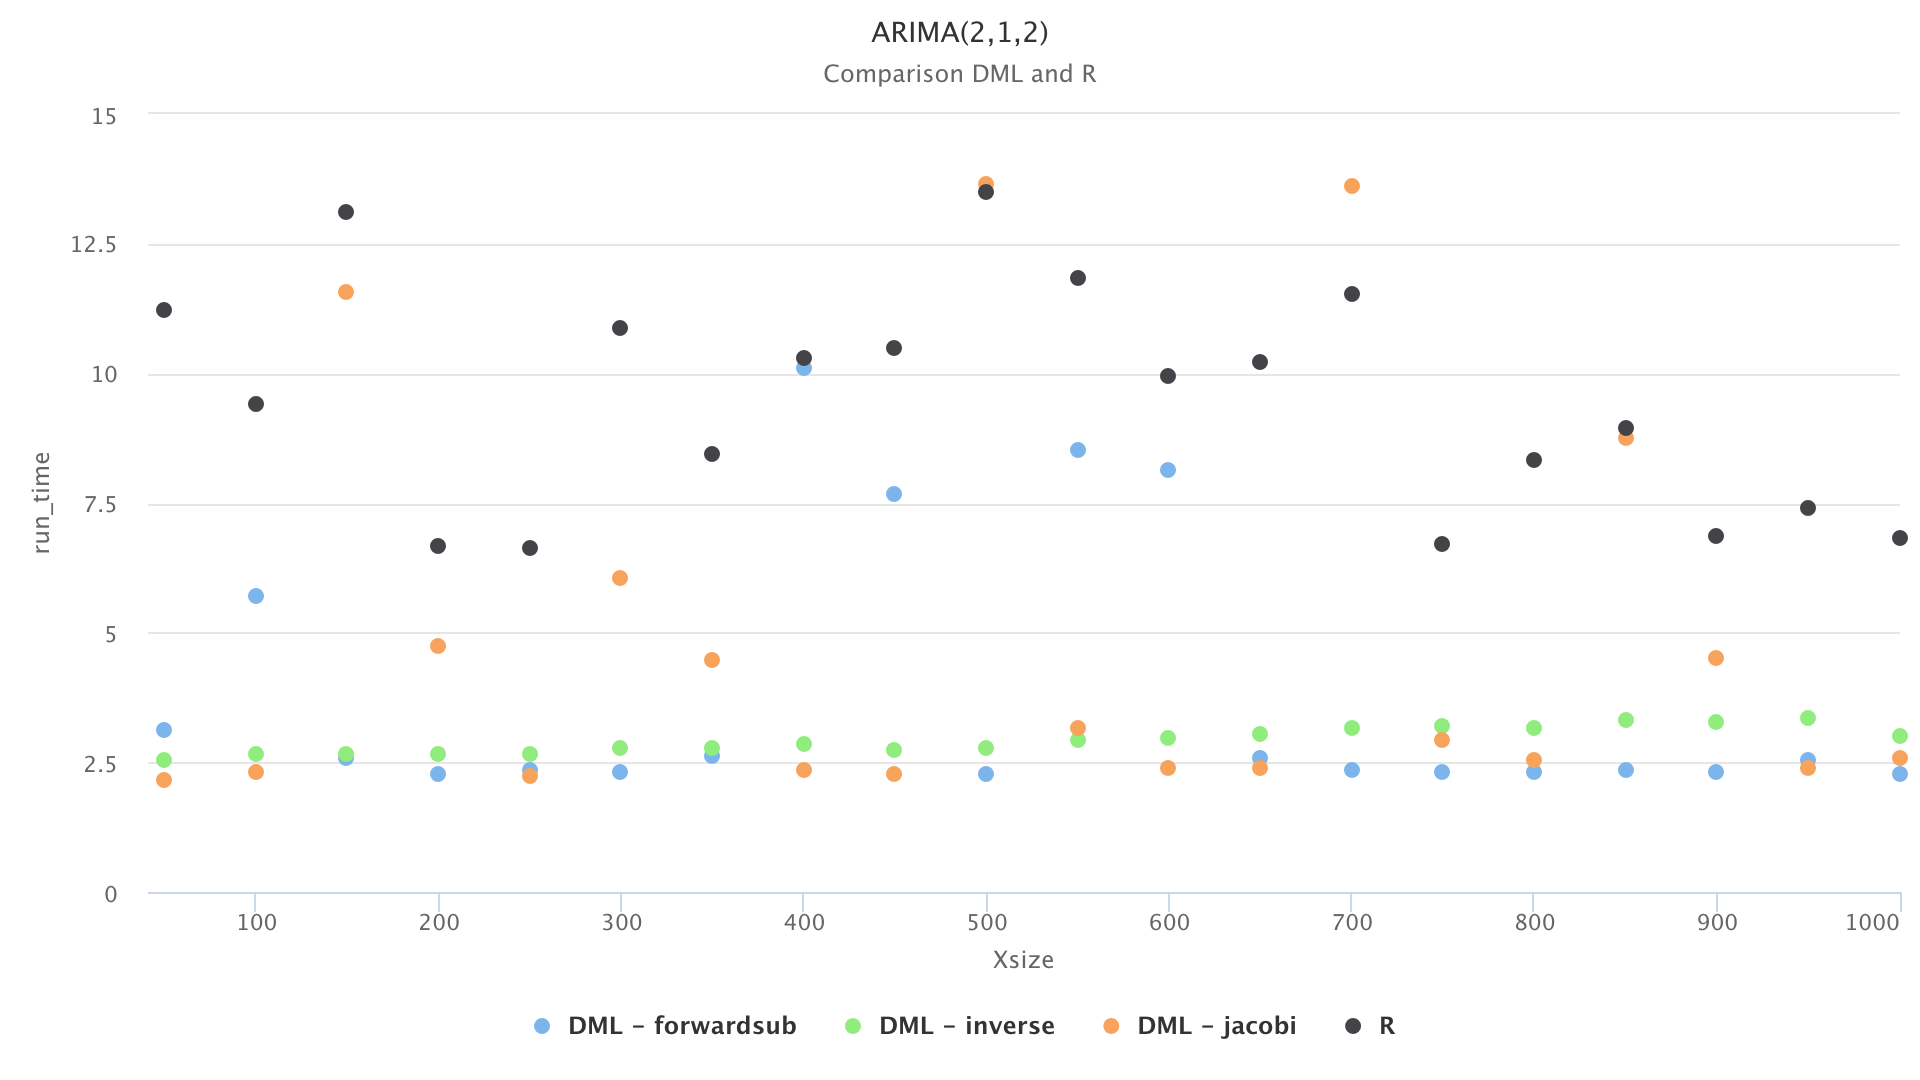
\includegraphics[width=\defaultsizeGraph]{images/arima212-runtime-scatter-all_small.png}}
	\caption{\textbf{Run time} of ARIMA(2,1,2) for DML and R for time series with sizes \textbf{from $50$ to $1,000$} }
    \label{apx-fig:arima212-runtime-scatter-all_small}
\end{figure}
	
	% Abkürzungsverzeichnis
	\cleardoublepage
	% !TeX root = ../dokumentation.tex

\addchap{\langabkverz}

\begin{acronym}
\acro{NASA}{National Aeronautics and Space Administration}
\acro{SMAP}{Soil Moisture Active Passive}
\acro{ARIMA}{Autoregressive Integrated Moving Average}
\acro{SARIMA}{Seasonal Autoregressive Integrated Moving Average}
\acro{SARMA}{Seasonal Autoregressive Moving Average}
\acro{ARMA}{Autoregressive Moving Average}
\acro{ARMAX}{Autoregressive Moving Average with exogenous inputs}
\acro{AR}{Autoregression}
\acro{SAR}{Seasonal Autoregression}
\acro{MA}{Moving Average}
\acro{SMA}{Seasonal Moving Average}
\acro{ML}{Maximum Likelihood}
\acro{DAG}{directed acyclic graph}
\acro{HOP}{high-level operation}
\acro{LOP}{low-level operation}
\acro{BFGS}{Broyden-Fletcher–Goldfarb-Shanno}
\acro{L-BFGS}{Limited-memory Broyden-Fletcher–Goldfarb-Shanno}
\acro{CG}{Conjugate Gradient}
\acro{Bi-CG}{Biconjugate Gradient}
\acro{CGS}{Conjugate Gradient Squared}
\acro{Bi-CGSTAB}{Biconjugate Gradient Stabilized}
\acro{GS}{Gauss-Seidel}
\acro{SOR}{Successive Over-Relaxation}
\acro{CSS}{Conditional Sum of Squares}
\acro{DML}{Declarative Machine Learning Language}
\acro{iid}{independent and identically
distributed}
\acro{API}{Application Programming Interface}
\acro{UDF}{User-Defined Function}
\acro{RMSE}{Root-Mean-Square Error}
\acro{JVM}{Java Virtual Machine}
\acro{HDFS}{Hadoop Distributed File System}
\acro{CSV}{Comma Seperated Values}


\end{acronym}
	
	% Literaturverzeichnis
	\cleardoublepage
	\printbibliography
	
\end{document}
